\documentclass[11pt,openany]{article}
\usepackage{mathtools, commath}
% Packages for formatting
\usepackage[margin=1in]{geometry}
\usepackage{fancyhdr}
\usepackage{enumerate}
\usepackage{graphicx}
\usepackage{kotex}
\usepackage{arydshln} % Include this package
\usepackage{bbding}
\usepackage{amsmath}
\usepackage{amsthm}
\usepackage[dvipsnames,table]{xcolor}
\usepackage{amssymb, amsfonts}
\usepackage{wasysym}
\usepackage{footnote}
\usepackage{tablefootnote}
\usepackage{arydshln} % Include this package
% Fonts
\usepackage[T1]{fontenc}
\usepackage[utf8]{inputenc}
\usepackage{newpxtext,newpxmath}
\usepackage{sectsty}

\usepackage{array}  % Load the array package

% Define a new column type 'L' for left alignment with a specified width
\newcolumntype{L}[1]{>{\raggedright\arraybackslash}p{#1}}

% Define colors
\definecolor{TealBlue1}{HTML}{0077c2}
\definecolor{TealBlue2}{HTML}{00a5e6}
\definecolor{TealBlue3}{HTML}{b3e0ff}
\definecolor{TealBlue4}{HTML}{00293c}
\definecolor{TealBlue5}{HTML}{e6f7ff}

\definecolor{thmcolor}{RGB}{231, 76, 60}
\definecolor{defcolor}{RGB}{52, 152, 219}
\definecolor{lemcolor}{RGB}{155, 89, 182}
\definecolor{corcolor}{RGB}{46, 204, 113}
\definecolor{procolor}{RGB}{241, 196, 15}

\usepackage{color,soul}
\usepackage{soul}
\newcommand{\mathcolorbox}[2]{\colorbox{#1}{$\displaystyle #2$}}
\usepackage{cancel}
\newcommand\crossout[3][black]{\renewcommand\CancelColor{\color{#1}}\cancelto{#2}{#3}}
\newcommand\ncrossout[2][black]{\renewcommand\CancelColor{\color{#1}}\cancel{#2}}

\usepackage{hyperref}
\usepackage{booktabs}

% Chapter formatting
\definecolor{titleTealBlue}{RGB}{0,53,128}
\usepackage{titlesec}
\titleformat{\section}
{\normalfont\sffamily\LARGE\bfseries\color{titleTealBlue!100!gray}}{\thesection}{1em}{}
\titleformat{\subsection}
{\normalfont\sffamily\Large\bfseries\color{titleTealBlue!75!gray}}{\thesubsection}{1em}{}
\titleformat{\subsubsection}
{\normalfont\sffamily\large\bfseries\color{titleTealBlue!50!gray}}{\thesubsubsection}{1em}{}

%Tcolorbox
\usepackage[most]{tcolorbox}
\usepackage{multirow}
\usepackage{multicol}

\usepackage{caption}

\usepackage[linesnumbered,ruled]{algorithm2e}
\usepackage{algpseudocode}
\usepackage{setspace}
\SetKwComment{Comment}{/* }{ */}
\SetKwProg{Fn}{Function}{:}{end}
\SetKw{End}{end}
\SetKw{DownTo}{downto}

% Define a new environment for algorithms without line numbers
\newenvironment{algorithm2}[1][]{
	% Save the current state of the algorithm counter
	\newcounter{tempCounter}
	\setcounter{tempCounter}{\value{algocf}}
	% redefine the algorithm numbering (remove prefix)
	\renewcommand{\thealgocf}{}
	\begin{algorithm}
	}{
	\end{algorithm}
	% Restore the algorithm counter state
	\setcounter{algocf}{\value{tempCounter}}
}

\usepackage{adjustbox}
% Header and footer formatting
\pagestyle{fancy}
\fancyhead{}
\fancyhf{}
\lhead{\textcolor{TealBlue2}{\large\textbf{Crypto \& Security Engineering Lab}}}
\rhead{\textcolor{TealBlue2}{\large\textbf{[Research] Jasmin Language}}}%\rule{3cm}{0.4pt}}
% Define footer
%\newcommand{\footer}[1]{
%\begin{flushright}
%	\vspace{2em}
%	\includegraphics[width=2.5cm]{school_logo.jpg} \\
%	\vspace{1em}
%	\textcolor{TealBlue2}{\small\textbf{#1}}
%\end{flushright}
%}
%\rfoot{\large Department of Information Security, Cryptogrphy and Mathematics, Kookmin Uni.\includegraphics[height=1.5cm]{school_logo.jpg}}
\fancyfoot{}
\fancyfoot[C]{-\thepage-}

\usepackage{tabularx}
\usepackage{longtable}
\usepackage{array}
\usepackage{tcolorbox}
\tcbset{colback=white, arc=5pt}

\definecolor{defcolor}{RGB}{52, 152, 219}
\definecolor{procolor}{RGB}{241, 196, 15}
\definecolor{thmcolor}{RGB}{231, 76, 60}
\definecolor{lemcolor}{RGB}{155, 89, 182}
\definecolor{corcolor}{RGB}{46, 204, 113}
\definecolor{execolor}{RGB}{90, 128, 127}

% Define a new command for the custom tcolorbox
\newcommand{\defbox}[2][]{%
	\begin{tcolorbox}[colframe=defcolor, title={\color{white}\bfseries #1}]
		#2
	\end{tcolorbox}
}

\newcommand{\lembox}[2][]{%
	\begin{tcolorbox}[colframe=lemcolor, title={\color{white}\bfseries #1}]
		#2
	\end{tcolorbox}
}

\newcommand{\probox}[2][]{%
	\begin{tcolorbox}[colframe=procolor, title={\color{white}\bfseries #1}]
		#2
	\end{tcolorbox}
}

\newcommand{\thmbox}[2][]{%
	\begin{tcolorbox}[colframe=thmcolor, title={\color{white}\bfseries #1}]
		#2
	\end{tcolorbox}
}

\newcommand{\corbox}[2][]{%
	\begin{tcolorbox}[colframe=corcolor, title={\color{white}\bfseries #1}]
		#2
	\end{tcolorbox}
}
\usepackage{listings}
\definecolor{keyword}{HTML}{8e4e9e}
\definecolor{myblue}{HTML}{3471d8}
\definecolor{type}{HTML}{4EC9B0}
\definecolor{golden}{HTML}{d19a66}

% Change "Listing" to another name, e.g., "Code"
\renewcommand{\lstlistingname}{Code}
\lstdefinestyle{normal}{
%	frame=single, % Border
%	basicstyle=\tt\small, % Code font style
%	breaklines=true, % Break long lines into multiple lines automatically
%	aboveskip=1.5\baselineskip, % Vertical whitespace before the listing
	tabsize=3, % How many space to a tab
	upquote=true,
	mathescape=false,
	columns=fullflexible,
	keepspaces=true,
	captionpos=b,
	frame=tb,
	rangebeginprefix={(**\ begin\ },
	rangeendprefix={(**\ end\ },
	rangesuffix={\ *)},
	includerangemarker=false,
	basicstyle=\small\ttfamily,
	identifierstyle={},
	keywordstyle=[1]{\bfseries\color{violet}},
	keywordstyle=[2]{\bfseries\color{olive}},
	keywordstyle=[3]{\bfseries\color{blue}},
	keywordstyle=[4]{\bfseries\color{blue}},
	keywordstyle=[5]{\bfseries\color{red}},
	keywordstyle=[6]{\bfseries\color{violet}},
}
\lstdefinestyle{c}{
	language=C,
	basicstyle=\ttfamily\small,        % Basic font style
	keywordstyle=\color{keyword}\bfseries,       % Keywords in bold blue
	keywordstyle=[2]\color{myblue}\bfseries,
	keywordstyle=[3]\color{magenta}\bfseries,
	keywordstyle=[4]\color{purple}\bfseries,
	stringstyle=\color{red!70},               % Strings in reddish color
	commentstyle=\color{green!50!black}\itshape, % Comments in italic green-black
	numberstyle=\tiny\color{gray},            % Line numbers in tiny gray font
	numbers=left,                             % Line numbers on the left
	stepnumber=1,                             % Number every line
	numbersep=8pt,                            % Space between line numbers and code
%	backgroundcolor=\color{gray!10},          % Light gray background
	frame=single,                             % Single-line frame around the code
	rulecolor=\color{gray},                   % Frame color
	tabsize=4,                                % Tab space width
	showstringspaces=false,                   % Don't show spaces in strings
	breaklines=true,                          % Line breaking enabled
	breakatwhitespace=true,                   % Break lines at whitespace
	captionpos=b,                             % Caption below the code
	escapeinside={\%*}{*)},                   % Allow LaTeX within code
	morekeywords={printf, scanf, main, size_t, uint8_t, uint16_t, uint32_t, uint64_t},
	morekeywords=[2]{randomSeed, hashArray,
	expandChallenge, expandATF_vec_copy, expandColumns, expandSeeds,
	invertingOnATF, actingOnATFS, columnsMatrix, columnsDecomposition,
	multiplicationModuloP, addmul_P32_into_64, reductionModuloP,
	reductionStrict, inversionModuloP},
	morekeywords=[3]{crypto_sign_keypair, crypto_sign},
	morekeywords=[4]{lu}
}
% Command to Include Rust Code
\newcommand{\ccode}[2][]{%
	\lstinputlisting[style=c,#1]{#2}
}

% Inline Code Highlighting
\newcommand{\cinline}[1]{%
	\lstinline[style=c]|#1|%
}
\lstdefinestyle{asm}{
	%	language=[x86masm]Assembler,
	language=C,
	basicstyle=\ttfamily\small,
	keywordstyle=\color{blue},
	commentstyle=\color{gray!50},
	stringstyle=\color{orange},
	morekeywords={.data, .align, .asciz, .text, .global, .type, .size, .extern, stp, mov, adr, ldr, add, bl, ret, ldp, and,
	movk, lsr, mul, sub, uxtw, cmp, blt, str, cbnz},
	numbers=none,
	frame=single,                             % Single-line frame around the code
	rulecolor=\color{gray},                   % Frame color
}

%\lstdefinestyle{jasmin}{
%	language=[x86masm]Assembler, % Closest to Jasmin syntax
%	basicstyle=\ttfamily\small, % Monospace font for code
%	keywordstyle=\color{blue}\bfseries, % Keywords in blue and bold
%	stringstyle=\color{orange}, % Strings in orange
%	commentstyle=\color{green!60!black}\itshape, % Comments in green
%	numbers=left, % Line numbers on the left
%	numberstyle=\tiny\color{gray}, % Line number style
%	stepnumber=1, % Show every line number
%	numbersep=5pt, % Space between numbers and code
%	frame=single, % Single frame around code
%	tabsize=4, % Tab width
%	showstringspaces=false, % Don't underline spaces in strings
%	breaklines=true, % Wrap long lines
%	captionpos=b, % Caption at the bottom
%	morekeywords={mov, add, sub, mul, xor, and, or, shl, shr, call, ret, lea}, % Add Jasmin-specific keywords
%	escapeinside={(*@}{@*)} % For embedding LaTeX inside code
%}



%
%% --------------------------------------------------------------------
%\newcommand{\dslash}{\mathbin{\mathsf{/\mkern-4mu/}}}
%\newcommand{\dslasheq}{\mathbin{\mathsf{/\mkern-4mu/\mkern-8mu=}}}
%\newcommand{\slasheq}{\mathbin{\mathsf{/\mkern-6mu=}}}

% --------------------------------------------------------------------
\definecolor{OliveGreen}{rgb}{0.33, 0.5, 0.18}
\definecolor{Blue}{rgb}{0.06, 0.2, 0.65}
\definecolor{grey}{rgb}{0.43, 0.5, 0.5}
\lstdefinestyle{jasmin}{
	mathescape=true,
	columns=fullflexible,
	keepspaces=true,
	captionpos=b,
	frame=tb,
%	xleftmargin=.1\textwidth,
%	xrightmargin=.1\textwidth,
	rangebeginprefix={(**\ begin\ },
	rangeendprefix={(**\ end\ },
	rangesuffix={\ *)},
	includerangemarker=false,
	basicstyle=\small\sffamily,
	identifierstyle={},
	keywordstyle=[1]{\color{OliveGreen}},
	keywordstyle=[2]{\color{keyword}\bfseries},
	keywordstyle=[3]{\color{Blue}},
	keywordstyle=[4]{\bfseries\color{OliveGreen}},
	keywordstyle=[5]{\color{Red}},
	keywordstyle=[6]{\color{golden}},
	keywordstyle=[7]{\bfseries\color{magenta}},
%	morekeywords=[7]{xor, aes, enc, dec},
	morekeywords=[2]{fn,for,to,downto,if,else,do,while,return,param},
	morekeywords=[3]{u256,u128,u64,u32,u16,u8,bool,int},
	morekeywords=[1]{reg,stack,inline,export},
	comment=[l][\color{grey}]{//},
	morecomment=[s][\color{grey}]{/*}{*/},
	alsoletter ={_},
	literate=
	{-}{-}{1}%
	{->}{$\rightarrow$}{1}%
	{4u64}{4u64}{1}%
	{>>}{$\gg$}{1}%
	{<<}{$\ll$}{1}%,
}[keywords,comments]
\newcommand{\jasmincode}[2][]{%
	\lstinputlisting[style=jasmin,#1]{#2}
}
\newcommand{\jasmininline}[1]{%
	\lstinline[style=jasmin]|#1|%
}

\newcommand{\dslash}{\mathbin{\mathsf{/\mkern-4mu/}}}
\newcommand{\dslasheq}{\mathbin{\mathsf{/\mkern-4mu/\mkern-8mu=}}}
\newcommand{\slasheq}{\mathbin{\mathsf{/\mkern-6mu=}}}
\newcommand{\drarrow}{\raisebox{.07em}{$\mathbin{\scriptstyle\mathsf{-\mkern-3mu>}}$}}
\newcommand{\dlarrow}{\raisebox{.07em}{$\mathbin{\scriptstyle\mathsf{<\mkern-3mu-}}$}}
\newcommand{\drrarrow}{\raisebox{.07em}{$\mathbin{\scriptstyle\mathsf{-\mkern-3mu>\mkern-3mu>}}$}}
\newcommand{\dllarrow}{\raisebox{.07em}{$\mathbin{\scriptstyle\mathsf{<\mkern-3mu<\mkern-3mu-}}$}}
\lstdefinestyle{easycrypt}{
	upquote=true,
%	escapechar=\#,
	mathescape=false,
	columns=fullflexible,
	keepspaces=true,
	captionpos=b,
	frame=tb,
%	xleftmargin=.1\textwidth,
%	xrightmargin=.1\textwidth,
	rangebeginprefix={(**\ begin\ },
	rangeendprefix={(**\ end\ },
	rangesuffix={\ *)},
	includerangemarker=false,
	basicstyle=\small\ttfamily,
	identifierstyle={},
	keywordstyle=[1]{\bfseries\color{violet}},
	keywordstyle=[2]{\bfseries\color{olive}},
	keywordstyle=[3]{\bfseries\color{blue}},
	keywordstyle=[4]{\bfseries\color{blue}},
	keywordstyle=[5]{\bfseries\color{red}},
	keywordstyle=[6]{\bfseries\color{violet}},
	morekeywords=[1]{arg},
	morecomment=[n][\itshape]{(*}{*)},
	morecomment=[n][\bfseries]{(**}{*)},
	morekeywords=[1]{forall,exists,fun,glob,let,in,var,proc,if,then,else,elif,while,assert,return,res,equiv,hoare,phoare,islossless,async},
	morekeywords=[2]{axiom,axiomatized,lemma,realize,proof,qed,abort,goal,end,import,export,include,local,declare,hint,nosmt,module,of,const,op,pred,inductive,notation,abbrev,require,theory,abstract,section,type,class,instance,print,search,as,Pr,clone,with,rename,prover,timeout,why3,dump,remove,Top,Self},
	morekeywords=[3]{beta,iota,zeta,eta,logic,delta,simplify,congr,change,split,left,right,case,pose,cut,have,suff,elim,clear,wlog,apply,rewrite,rwnormal,subst,progress,trivial,auto,idtac,move,modpath,field,fieldeq,ring,ringeq,algebra,replace,transitivity,symmetry,seq,wp,sp,sim,skip,call,rcondt,rcondf,swap,cfold,rnd,pr_bounded,bypr,byphoare,byequiv,fel,conseq,exfalso,inline,alias,fission,fusion,unroll,splitwhile,kill,eager},
	morekeywords=[4]{try,first,last,do,strict,expect},
	morekeywords=[5]{exact,assumption,smt,by,reflexivity,done,solve},
	morekeywords=[6]{admit,admitted},
	literate=
	{tau}{$\tau$}1
	{sigma}{$\sigma$}1
	% note double "_" below
	% in actual EasyCrypt examples, do not use __
	% in specifications, these are rendered as subscripts
	{__1}{${}_{\!1}$}1
	{__2}{${}_{\!2}$}1
	{__3}{${}_{\!3}$}1
	{__n}{${}_{\!n}$}1
	{__p}{${}_{\!p}$}1
	{,,,}{$\mathrel{\ldots}$}1
	{...}{$\mathrel{\cdots}$}1
	{->}{$\drarrow$}1
	{<-}{$\dlarrow$}1
	{->>}{$\drrarrow$}2
	{<<-}{$\dllarrow$}2
}
\newcommand{\easycryptcode}[2][]{%
	\lstinputlisting[style=easycrypt,#1]{#2}
}
\newcommand{\easycryptinline}[1]{%
	\lstinline[style=easycrypt]|#1|%
}
\newcommand{\eccode}[2][]{%
	\lstinputlisting[style=easycrypt,#1]{#2}
}
\newcommand{\ecinline}[1]{%
	\lstinline[style=easycrypt]|#1|%
}

%\lstdefinestyle{easycrypt}{
%	language=ML, % EasyCrypt syntax is close to ML
%	basicstyle=\ttfamily\small, % Monospace font for code
%	keywordstyle=\color{purple}\bfseries, % Keywords in purple and bold
%	commentstyle=\color{green!60!black}, % Comments in green
%	stringstyle=\color{orange}, % Strings in orange
%	numbers=left, % Line numbers on the left
%	numberstyle=\tiny\color{gray}, % Line number style
%	stepnumber=1, % Show every line number
%	numbersep=5pt, % Space between numbers and code
%	frame=single, % Single frame around code
%	tabsize=4, % Tab width
%	showstringspaces=false, % Don't underline spaces in strings
%	breaklines=true, % Wrap long lines
%	captionpos=b, % Caption at the bottom
%	morekeywords={module, axiom, lemma, theorem, proof, qed, fun, let, in, forall, exists, if, then, else, return, assume, while, do, match, with}, % EasyCrypt-specific keywords
%	escapeinside={(*@}{@*)} % For embedding LaTeX inside code
%}
%\newcommand{\easycryptcode}[2][]{%
%	\lstinputlisting[style=easycrypt,#1]{#2}
%}
%\newcommand{\easycryptinline}[1]{%
%	\lstinline[style=easycrypt]|#1|%
%}
\usepackage{amsthm}

% Define custom theorem styles
\newtheoremstyle{dotless} % Name of the style
{3pt} % Space above
{3pt} % Space below
{\itshape} % Body font
{} % Indent amount
{\bfseries} % Theorem head font
{} % Punctuation after theorem head
{2.5mm} % Space after theorem head
{} % Theorem head spec

\newtheoremstyle{definitionstyle} % Name of the style
{3pt} % Space above
{3pt} % Space below
{} % Body font
{} % Indent amount
{\bfseries} % Theorem head font
{.} % Punctuation after theorem head
{2.5mm} % Space after theorem head
{} % Theorem head spec

% Applying custom styles
%\theoremstyle{dotless}
\newtheorem{theorem}{Theorem} % Theorem environment with section-wise numbering
\newtheorem*{theorem*}{Theorem} % Theorem environment with section-wise numbering
\newtheorem*{proposition*}{Proposition} % Theorem environment with section-wise numbering
\newtheorem*{corollary*}{Corollary} % Theorem environment with section-wise numbering
\newtheorem{proposition}[theorem]{Proposition} % Theorem environment with section-wise numbering
\newtheorem{lemma}[theorem]{Lemma} % Lemma shares the counter with theorem
\newtheorem{corollary}[theorem]{Corollary} % Corollary shares the counter with theorem

\theoremstyle{definitionstyle}
\newtheorem*{statement}{\textcolor{orange}{Statement}}
\newtheorem*{analysis}{\textcolor{magenta}{Analysis}}
\newtheorem*{pftactics}{\textcolor{teal}{Proof Tactics}}
\newtheorem*{observation}{\textcolor{Magenta}{Observation}}
\newtheorem{definition}{Definition} % Definition shares the counter with theorem
\newtheorem{example}{Example} % Example shares the counter with theorem
\newtheorem{exercise}{{Exercise}} % Example shares the counter with theorem
\newtheorem{remark}{Remark} % Remark shares the counter with theorem
\newtheorem*{note}{Note}

\newtheorem*{axiom*}{Axiom}
\newtheorem*{definition*}{Definition} % Definition shares the counter with theorem
\newtheorem*{example*}{Example} % Example shares the counter with theorem
\newtheorem*{exercise*}{\textcolor{violet}{Exercise}} % Example shares the counter with theorem
\newtheorem*{remark*}{Remark} % Remark shares the counter with theorem


\usepackage{tikz}
\usepackage{tikz-cd}
\usepackage{tikz-3dplot}
\def\Circlearrowleft{\ensuremath{%
		\rotatebox[origin=c]{180}{$\circlearrowleft$}}}
\def\Circlearrowright{\ensuremath{%
		\rotatebox[origin=c]{180}{$\circlearrowright$}}}
\def\CircleArrowleft{\ensuremath{%
		\reflectbox{\rotatebox[origin=c]{180}{$\circlearrowleft$}}}}
\def\CircleArrowright{\ensuremath{%
		\reflectbox{\rotatebox[origin=c]{180}{$\circlearrowright$}}}}
\usetikzlibrary{
	3d, % For 3D drawing
	angles,
	arrows,
	arrows.meta,
	backgrounds,
	bending,
	calc,
	decorations.pathmorphing,
	decorations.pathreplacing,
	decorations.markings,
	fit,
	matrix,
	patterns,
	patterns.meta,
	positioning,
	quotes,
	shadows,
	shapes,
	shapes.geometric,
	trees
}

\usepackage{pgfplots}
\pgfplotsset{compat=newest} % Adjust to your version of pgfplots
\usepgfplotslibrary{statistics}
% Commands for Research
\newcommand{\PRP}{\text{\normalfont PRP}}
\newcommand{\adversary}{\mathcal{A}}
\newcommand{\Adv}{\text{\normalfont Adv}}
\newcommand{\negl}{\text{\normalfont negl}}
\newcommand{\plaintext}{\mathcal{P}}
\newcommand{\messagespace}{\mathcal{M}}
\newcommand{\ciphertext}{\mathcal{C}}
\newcommand{\keyspace}{\mathcal{K}}
\newcommand{\encryption}{\mathcal{E}}
\newcommand{\decryption}{\mathcal{D}}
\newcommand{\nonce}{\mathcal{N}}
\newcommand{\keygen}{\mathsf{KeyGen}}
\newcommand{\enc}{\mathsf{Enc}}
\newcommand{\dec}{\mathsf{Dec}}
\newcommand{\uniform}{\xleftarrow{\$}}

% Commands for EasyCrypt
% Tools
\definecolor{eccolor}{HTML}{0f55bc}
\newcommand{\EasyCrypt}{{\bfseries\color{eccolor}\textsf{EasyCrypt}}\xspace}
\newcommand{\EC}{{\bfseries\color{eccolor}\textsf{EC}}\xspace}
\newcommand{\OCaml}{{\bfseries\textsf{OCaml}}\xspace}
\newcommand{\Emacs}{{\bfseries\textsf{Emacs}}\xspace}
\newcommand{\ZThree}{{\bfseries\textsf{Z3}}\xspace}
\newcommand{\CVCFour}{{\bfseries\textsf{CVC4}}\xspace}
\newcommand{\AltErgo}{{\bfseries\textsf{Alt-ergo}}\xspace}
\newcommand{\ProofGeneral}{{\bfseries\textsf{Proof General}}\xspace}
\newcommand{\CertiCrypt}{\textsf{CertiCrypt}\xspace}
\newcommand{\CertiPriv}{\textsf{CertiPriv}\xspace}
\newcommand{\SsReflect}{\textsf{SsReflect}\xspace}
\newcommand{\Coq}{{\bfseries\textsf{Coq}}\xspace}
\newcommand{\WhyThree}{{\bfseries\textsf{Why3}}\xspace}
\newcommand{\SMT}{{\bfseries\textsf{SMT}}\xspace}
% Languages and Logics
\newcommand{\pWHILE}{\textsf{p}\textsc{While}\xspace}
\newcommand{\pRHL}{\textsf{pRHL}\xspace}
% Version numbers
\newcommand{\ECversion}{1.0\xspace}
%% Misc
\newcommand{\DONE}{}% {{\color{red}DONE}}
\newcommand{\Example}{\paragraph*{Example}}
\newcommand{\Syntax}{\paragraph*{Syntax}}
\newcommand{\Description}{\paragraph*{Description}}
\newcommand{\INDRoR}{\textsf{IND-RoR}\xspace}
\newcommand{\INDCPA}{\textsf{IND-CPA}\xspace}
\newcommand{\INDCCAone}{\textsf{IND-CCA1}\xspace}
\newcommand{\INDCCA}{\textsf{IND-CCA}\xspace}
\newcommand{\EFCMA}{\textsf{EF-CMA}\xspace}
\newcommand{\LCDH}{\ensuremath{\mathsf{LCDH}}\xspace}
\newcommand{\CDH}{\textsf{CDH}\xspace}
\newcommand{\DDH}{\textsf{DDH}\xspace}
\newcommand{\ElGamal}{\textsf{ElGamal}\xspace}
\newcommand{\HElGamal}{\textsf{HElGamal}\xspace}
\newcommand{\RSA}{\textsf{RSA}\xspace}
\newcommand{\OAEP}{\textsf{OAEP}\xspace}
\newcommand{\FDH}{\textsf{FDH}\xspace}
\newcommand{\HMAC}{\textsf{HMAC}\xspace}
\newcommand{\CS}{\textsf{CS}\xspace}
\newcommand{\Skein}{\textsf{Skein}\xspace}
\newcommand{\TCR}{\textsf{TCR}\xspace}

\newcommand{\KG}{\mathcal{KG}}
\newcommand{\Enc}{\mathcal{E}}
\newcommand{\Dec}{\mathcal{D}}

%%% Complexity and termination
%\newcommand{\lossless}{\mathsf{lossless}}

%%% Sets
%\newcommand{\zeroone}{[0,1]}
%\newcommand{\bit}{\{0,1\}}
%\newcommand{\bitstring}[1]{\ensuremath{\bit^{#1}}}
%\newcommand{\bool}{\mathbb{B}}
%\newcommand{\nat}{\mathbb{N}}
%\newcommand{\real}{\mathbb{R}}
%\newcommand{\option}[1]{#1_\bot}
%
%%% Mathematics
%\newcommand{\conv}[1][]{\mathrel{\leftrightarrow^*_{#1}}}
%\renewcommand{\Pr}[2]{\mathrm{Pr}\left[#1 : #2\right]}
%\newcommand{\Prm}[3]{\mathrm{Pr}\left[#1,#3 : #2\right]}
%\newcommand{\labs}{\left\lvert}
%\newcommand{\rabs}{\right\rvert}
%\newcommand{\charfun}{\mathds{1}}

%% Distribution monad
%\newcommand{\supp}{\mathsf{support}}
%\newcommand{\range}[2]{\mathsf{range}~{#1}~{#2}}

%% Semantics 

% \newcommand{\sem}[1]{\llbracket #1 \rrbracket}
%\newcommand{\subst}[2]{\left[{}^{#2}/{}_{#1}\right]}
%\newcommand{\fv}{\mathsf{fv}}
%\newcommand{\modifies}{\mathsf{mod}}
%\newcommand{\glob}{\mathsf{glob}}
%\newcommand{\Env}{\mathcal{E}}

%%% Well-formed adversaries
%%% Program Judgements 
\newcommand{\Hoare}[3]{\left[{#1}:{#2}\Longrightarrow{#3}\right]}
%\newcommand{\Equiv}[4]{\left[{#1}\sim{#2}:{#3}\Longrightarrow{#4}\right]}
%\newcommand{\bdHoareS}[5]{{\Hoare{#1}{#2}{#3}}\,{#4}\,{#5}}
%\newcommand{\HoareLe}[4]{\bdHoareS{#1}{#2}{#3}{\leq}{#4}}
%\newcommand{\HoareEq}[4]{\bdHoareS{#1}{#2}{#3}{=}{#4}}
%\newcommand{\HoareGe}[4]{\bdHoareS{#1}{#2}{#3}{\geq}{#4}}
%
%
%% \newcommand{\Equiv}[4]{\models {#1} \sim {#2} : {#3} \Longrightarrow {#4}}
%% \newcommand{\AEquiv}[6]{\models {#2} \sim_{#5,#6} {#3} : {#1} \Longrightarrow {#4}}
%% \newcommand{\JAEquiv}[6]{{#2} \sim_{#5,#6} {#3} : {#1} \Longrightarrow {#4}}
%% \newcommand{\EquivMem}[2]{\models {#1} \equiv {#2}}
%% \newcommand{\EqObs}[4]{\models {#1} \simeq^{#3}_{#4} {#2}}
%% \newcommand{\AEqObs}[5]{\models {#1} \simeq^{#3}_{{#4}} {#2} \preceq {#5}} 
%% \newcommand{\ACEqObs}[7]
%%         {\AEqObs{\left[ #1 \right]_{#6}}{\left[ #2 \right]_{#7}}{#3}{#4}{#5}}
%% \newcommand{\Triple}[3]{\sem{#2} {#3} \preceq {#1}}
%% \newcommand{\DTriple}[3]{\sem{#2} {#3} \succeq {#1}}
%% \newcommand{\dequiv}[3]{{#1} \simeq_{#3} {#2}}
%% \newcommand{\fequiv}[3]{{#1} =_{#3} {#2}}
%% \newcommand{\Pre}{\Psi}
%% \newcommand{\Post}{\Phi}
%% \newcommand{\Inv}{\Phi}
%\newcommand{\side}[1]{\langle #1 \rangle}
%\newcommand{\sidel}{\side{1}}
%\newcommand{\sider}{\side{2}}
%% \newcommand{\eqobsin}{\mathsf{eqobs\_in}}
%% \newcommand{\eqobsout}{\mathsf{eqobs\_out}}
%\newcommand{\pre}{\Psi}
%\newcommand{\post}{\Phi}
%\newcommand{\bound}{\delta}
%\newcommand{\ECinsupp}[2]{\mathec{Distr.in_supp}\,{#1}\,{#2}}
%\newcommand{\insupp}[2]{{#1}\in\mathec{supp}\,{#2}}
%%% Variables
%
%% \newcommand{\LH}{\gl{L}_H}
%% \newcommand{\LD}{\gl{L}_\Dec}
%% \newcommand{\cdef}{\gl{\gamma_\mathsf{def}}}
%\newcommand{\var}[1]{\ensuremath{\mathit{#1}} \xspace}

%% Constants and operators
% TODO: Update!
%\newcommand{\true}{\mathsf{true}}
%\newcommand{\false}{\mathsf{false}}
%\newcommand{\nil}{\mathsf{nil}}
%\newcommand{\hd}{\mathsf{hd}}
%\newcommand{\tl}{\mathsf{tl}}
%\newcommand{\app}{\mathbin{+\mkern-7mu+}}
%\newcommand{\concat}{\parallel}
%\newcommand{\xor}{\oplus}
%\newcommand{\msb}[2]{[#1]^{#2}}
%\newcommand{\lsb}[2]{[#1]_{#2}}
%\newcommand{\dom}{\mathsf{dom}}
%\newcommand{\ran}{\mathsf{ran}}
%\newcommand{\fst}{\mathsf{fst}}
%\newcommand{\snd}{\mathsf{snd}}
%\newcommand{\some}[1]{#1}
%\newcommand{\none}{\bot}
%
%\newcommand{\Int}{\mathsf{Int}}
%\newcommand{\tint}{\mathsf{int}}
%
%\newcommand{\tbool}{\mathsf{bool}}


%
\newcommand{\plain}{\mathcal{P}}
\newcommand{\key}{\mathcal{K}}
\newcommand{\authen}{\mathcal{A}}
\newcommand{\signature}{\mathcal{S}}
\newcommand{\verification}{\mathcal{V}}
\newcommand{\sig}{\textbf{sig}}
\newcommand{\ver}{\textbf{ver}}

\newcommand{\ie}{\textnormal{i.e.}}
\newcommand{\rsa}{\mathsf{RSA}}
\newcommand{\rsacrt}{\mathsf{RSA}\textendash\mathsf{CRT}}
\newcommand{\inv}[1]{#1^{-1}}

%New Command
%\newcommand{\set}[1]{\left\{#1\right\}}
\newcommand{\N}{\mathbb{N}}
\newcommand{\Z}{\mathbb{Z}}
\newcommand{\Q}{\mathbb{Q}}
\newcommand{\R}{\mathbb{R}}
\newcommand{\cR}{\mathcal{R}}
\newcommand{\C}{\mathbb{C}}
\newcommand{\F}{\mathbb{F}}
\newcommand{\nbhd}{\mathcal{N}}
\newcommand{\Log}{\operatorname{Log}}
\newcommand{\Arg}{\operatorname{Arg}}
\newcommand{\pv}{\operatorname{P.V.}}

\newcommand{\of}[1]{\left( #1 \right)} 
%\newcommand{\abs}[1]{\left\lvert #1 \right\rvert}
%\newcommand{\norm}[1]{\left\| #1 \right\|}

\newcommand{\sol}{\textcolor{magenta}{\bf Sol}}

\DeclarePairedDelimiter\ceil{\lceil}{\rceil}
\DeclarePairedDelimiter\floor{\lfloor}{\rfloor}


\newcommand{\cyclic}[1]{\langle #1 \rangle}
\newcommand{\xmark}{\textcolor{red}{\XSolidBrush}}
\newcommand{\vmark}{\textcolor{green!75!black}{\CheckmarkBold}}

\newcommand{\gen}[1]{\langle #1 \rangle}
\newcommand{\Gen}[1]{\left\langle #1 \right\rangle}

\newcommand{\img}[1]{\text{Img}(#1)}
\newcommand{\Img}[1]{\text{Img}\left(#1\right)}
\newcommand{\preimg}[1]{\text{Img}^{-1}(#1)}
\newcommand{\Preimg}[1]{\text{Img}^{-1}\left(#1\right)}

\newcommand{\relation}{\mathrel{\mathcal{R}}}
\newcommand{\injection}{\rightarrowtail}
\newcommand{\surjection}{\twoheadrightarrow}
\newcommand{\id}{\textnormal{id}}

\newcommand{\eqclass}[1]{\left[#1\right]}

% Define custom colors for O and X
\newcommand{\yes}{\textcolor{blue}{\bf \fullmoon}}
\newcommand{\no}{\textcolor{red}{\bf \texttimes}}

\usepackage{proof}
\usepackage{simplebnf}

\usepackage{background}  % For setting background images
%% Background settings for the title page
%\backgroundsetup{
%	scale=4,  % Scale the image to fit the page
%	color=black,  % Keep the image colors unchanged
%	opacity=.05,  % Fully opaque (1.0)
%	angle=0,  % No rotation
%%	position=current page.south,  % Position relative to the page
%	vshift=0cm,  % Vertical shift
%	hshift=0cm,  % Horizontal shift
%	contents={
\includegraphics[scale=1]{images/school-logo}} % Background image path
%}
% Background settings (only for the title page)
\backgroundsetup{
	scale=1,  % Scale the image to fit the page
	color=black,  % Keep the image color as is
	opacity=.1,  % Fully opaque background
	angle=0,  % No rotation
%	position=current page.south,  % Align to bottom of the page
	vshift=1cm,  % Adjust vertical alignment if needed
%	hshift=0cm,  % Adjust horizontal alignment if needed
	contents={}
}
% Command to set background for title page
\newcommand{\setPageBackground}{
	\backgroundsetup{
		contents={
\includegraphics[scale=4]{images/school-logo}
%		contents={
\includegraphics[width=\paperwidth,height=\paperheight]{images/school-logo}
		} % Replace with your image
	}
}

\usepackage{csquotes}
\setstretch{1.25}
\begin{document}
\begin{titlepage}
\setPageBackground  % Enable background image for title page
\begin{center}
	{\Huge{\textbf{A Commentary for\\ ``The Joy of EasyCrypt''}}\par}
	\vspace{0.05cm}
	\LARGE\textit{A Beginner’s Guide to Formal Verification of Cryptography}\\
	\vspace{.5cm}
	{\LARGE\textbf{v 1.0}\par}
	\vspace{.5in}
	{\LARGE {\textbf{Ji, Yong-hyeon}\\ (\texttt{hacker3740@kookmin.ac.kr})}\par}
%	\vspace{1.5in}
%	
\includegraphics[scale=.35]{images/school-logo-opa5}\par
%	\vspace{.25in}
	\vfill
	{\Large\bf \textsf{Department of Information Security, Cryptology, and Mathematics}\par}
	{\Large\textsf{College of Science and Technology}\par}
	{\Large\textsf{Kookmin University}\par}
	\vspace{.75in}
	
\includegraphics[scale=.35]{images/logo.png}\par
	\vspace{.25in}
	{\Large\textsf{\today}\par}
\end{center}
\end{titlepage}
\newpage

\vfill
\subsection*{Copyright}
%\large
\textcopyright~ 2024 Crypto and Security Engineering Lab
All rights reserved.

This document and its content are the intellectual property of ``Ji, Yong-hyeon''. No part of this document may be reproduced, distributed, or transmitted in any form or by any means, including photocopying, recording, or other electronic or mechanical methods, without the prior written permission of the author, except in the case of brief quotations embodied in critical reviews and certain other noncommercial uses permitted by copyright law. For permission requests, write to the author at the e-mail.

\vfill
\subsection*{Changelog}
\large
\begin{tabular}{@{} L{0.05\textwidth} L{0.2\textwidth} L{0.7\textwidth} @{}} % Column widths specified here, change as needed for your content
	\toprule
	v1.0 & 2025-01-20 & Initial release: \\%Implementation and benchmarks.\\
	%		v1.1 & 20XX-02-27 & Pellentesque iaculis odio vel nisl ullamcorper, nec faucibus ipsum molestie.\\
	%		v1.2 & 20XX-03-15 & Sed dictum nisl non aliquet porttitor.\\
	\bottomrule
\end{tabular}

\newpage

\pagenumbering{arabic}
\tableofcontents
\newpage
\section{Computer-Aided Cryptography}
%\subsection{Introduction to Computer-aided Cryptography}
\begin{center}
	\enquote{To define is to limit.}
\end{center}
\begin{flushright}
	--- Oscar Wilde
\end{flushright}
%This statement reflects the idea that definitions can impose boundaries on understanding. Boundaries are inherent to understanding. In the realm of cryptography, this truth resonates deeply, as each definition we craft frames the scope of what we can secure and protect. By limiting our focus to specific, well-characterized challenges, cryptography empowers us to construct rigorous, mathematically sound assurances against precise threats. Yet, this act of defining also confines, leaving the untamed complexity of reality beyond its reach. It is within these limits that cryptography achieves its most profound victories, not by claiming to address every possibility, but by offering clarity and reliability in the face of clearly articulated dangers. In the spirit of Wilde's insight, we embrace these limits, for it is through them that the discipline achieves its elegance and utility.
This statement reflects the idea that definitions can impose boundaries on understanding. Boundaries are inherent to understanding, as they help us simplify and categorize complex ideas. In cryptography, these boundaries take the form of precisely defined problems, enabling us to address specific challenges with mathematical rigor. However, this act of definition also constrains us, leaving out the nuances of the real world. Cryptography thrives within these limits, offering clarity and certainty within a structured framework while acknowledging the complexities that exist beyond.\par
Modern cryptography deals with three main problems related to the security of communication.
\begin{enumerate}
	\item \textbf{Privacy}:  Protecting information from being accessed by unauthorised parties.
	\item \textbf{Integrity}: Protecting information from being tampered with or altered
	\item \textbf{Authenticity}: Making sure the information is from an authentic source
\end{enumerate}
Each of these properties can be defined as a mathematical property of information,
and claiming that a cryptographic protocol protects a certain property is equivalent to proving that the information possesses that mathematical property. Given that the proofs
can be complicated and hard to follow, the idea of using computers to verify the proofs comes in here.\par
The tools for computer-aided cryptography come in different flavours based on what
is being dealt with. Broadly speaking, the tools are developed for the following
\begin{enumerate}
	\item \textbf{Design-level security}: To reason about the design of a protocol
	\item \textbf{Functional correctness and efficiency}: To formalise that the implementations match the designs
	\item \textbf{Implementation-level security}: To make sure that the implementations do not have other security risks
\end{enumerate}
Designing cryptographic systems without established methodologies is a perilous endeavor fraught with intricate pitfalls. Flawed security proofs, often born from misconstrued assumptions, undermine the theoretical foundation of a system's resilience. Buggy implementations further exacerbate the issue, introducing subtle vulnerabilities that unravel the integrity of even the most robust designs. Adding to the conundrum are pesky side-channels, the unanticipated vectors through which adversaries extract sensitive data by exploiting timing, power consumption, or electromagnetic emissions. Together, these challenges make rolling your own cryptography a veritable minefield.\par
In contemporary practice, the cryptographic community has developed a symbiotic triad of methods to combat these challenges. First, security proofs are meticulously composed using pen and paper, with each step scrutinized to ensure resilience against clearly articulated threat models. Next, implementations are subjected to rigorous testing and thorough code audits to unearth and rectify latent flaws. Finally, developers employ the art of crafting ``constant-time'' code, a technique designed to thwart side-channel attacks by eliminating variations in execution time that could reveal secrets. While these methods represent significant progress, they remain reliant on human precision and judgment.\par
The future of cryptographic assurance lies in delegating critical tasks to computational systems, enabling unprecedented rigor and reliability. Machine-checked security proofs leverage formal verification to eliminate human error, ensuring that theoretical guarantees are watertight. Verification extends to the implementation layer, where tools validate the safety and correctness of code, bridging the gap between abstract design and real-world execution. Moreover, automated analysis ensures adherence to ``constant-time'' principles, offering robust defenses against side-channel exploitation. By intertwining human ingenuity with computational exactitude, this approach heralds a paradigm shift in cryptographic design and validation.
\begin{center}\adjustbox{width=\textwidth}{
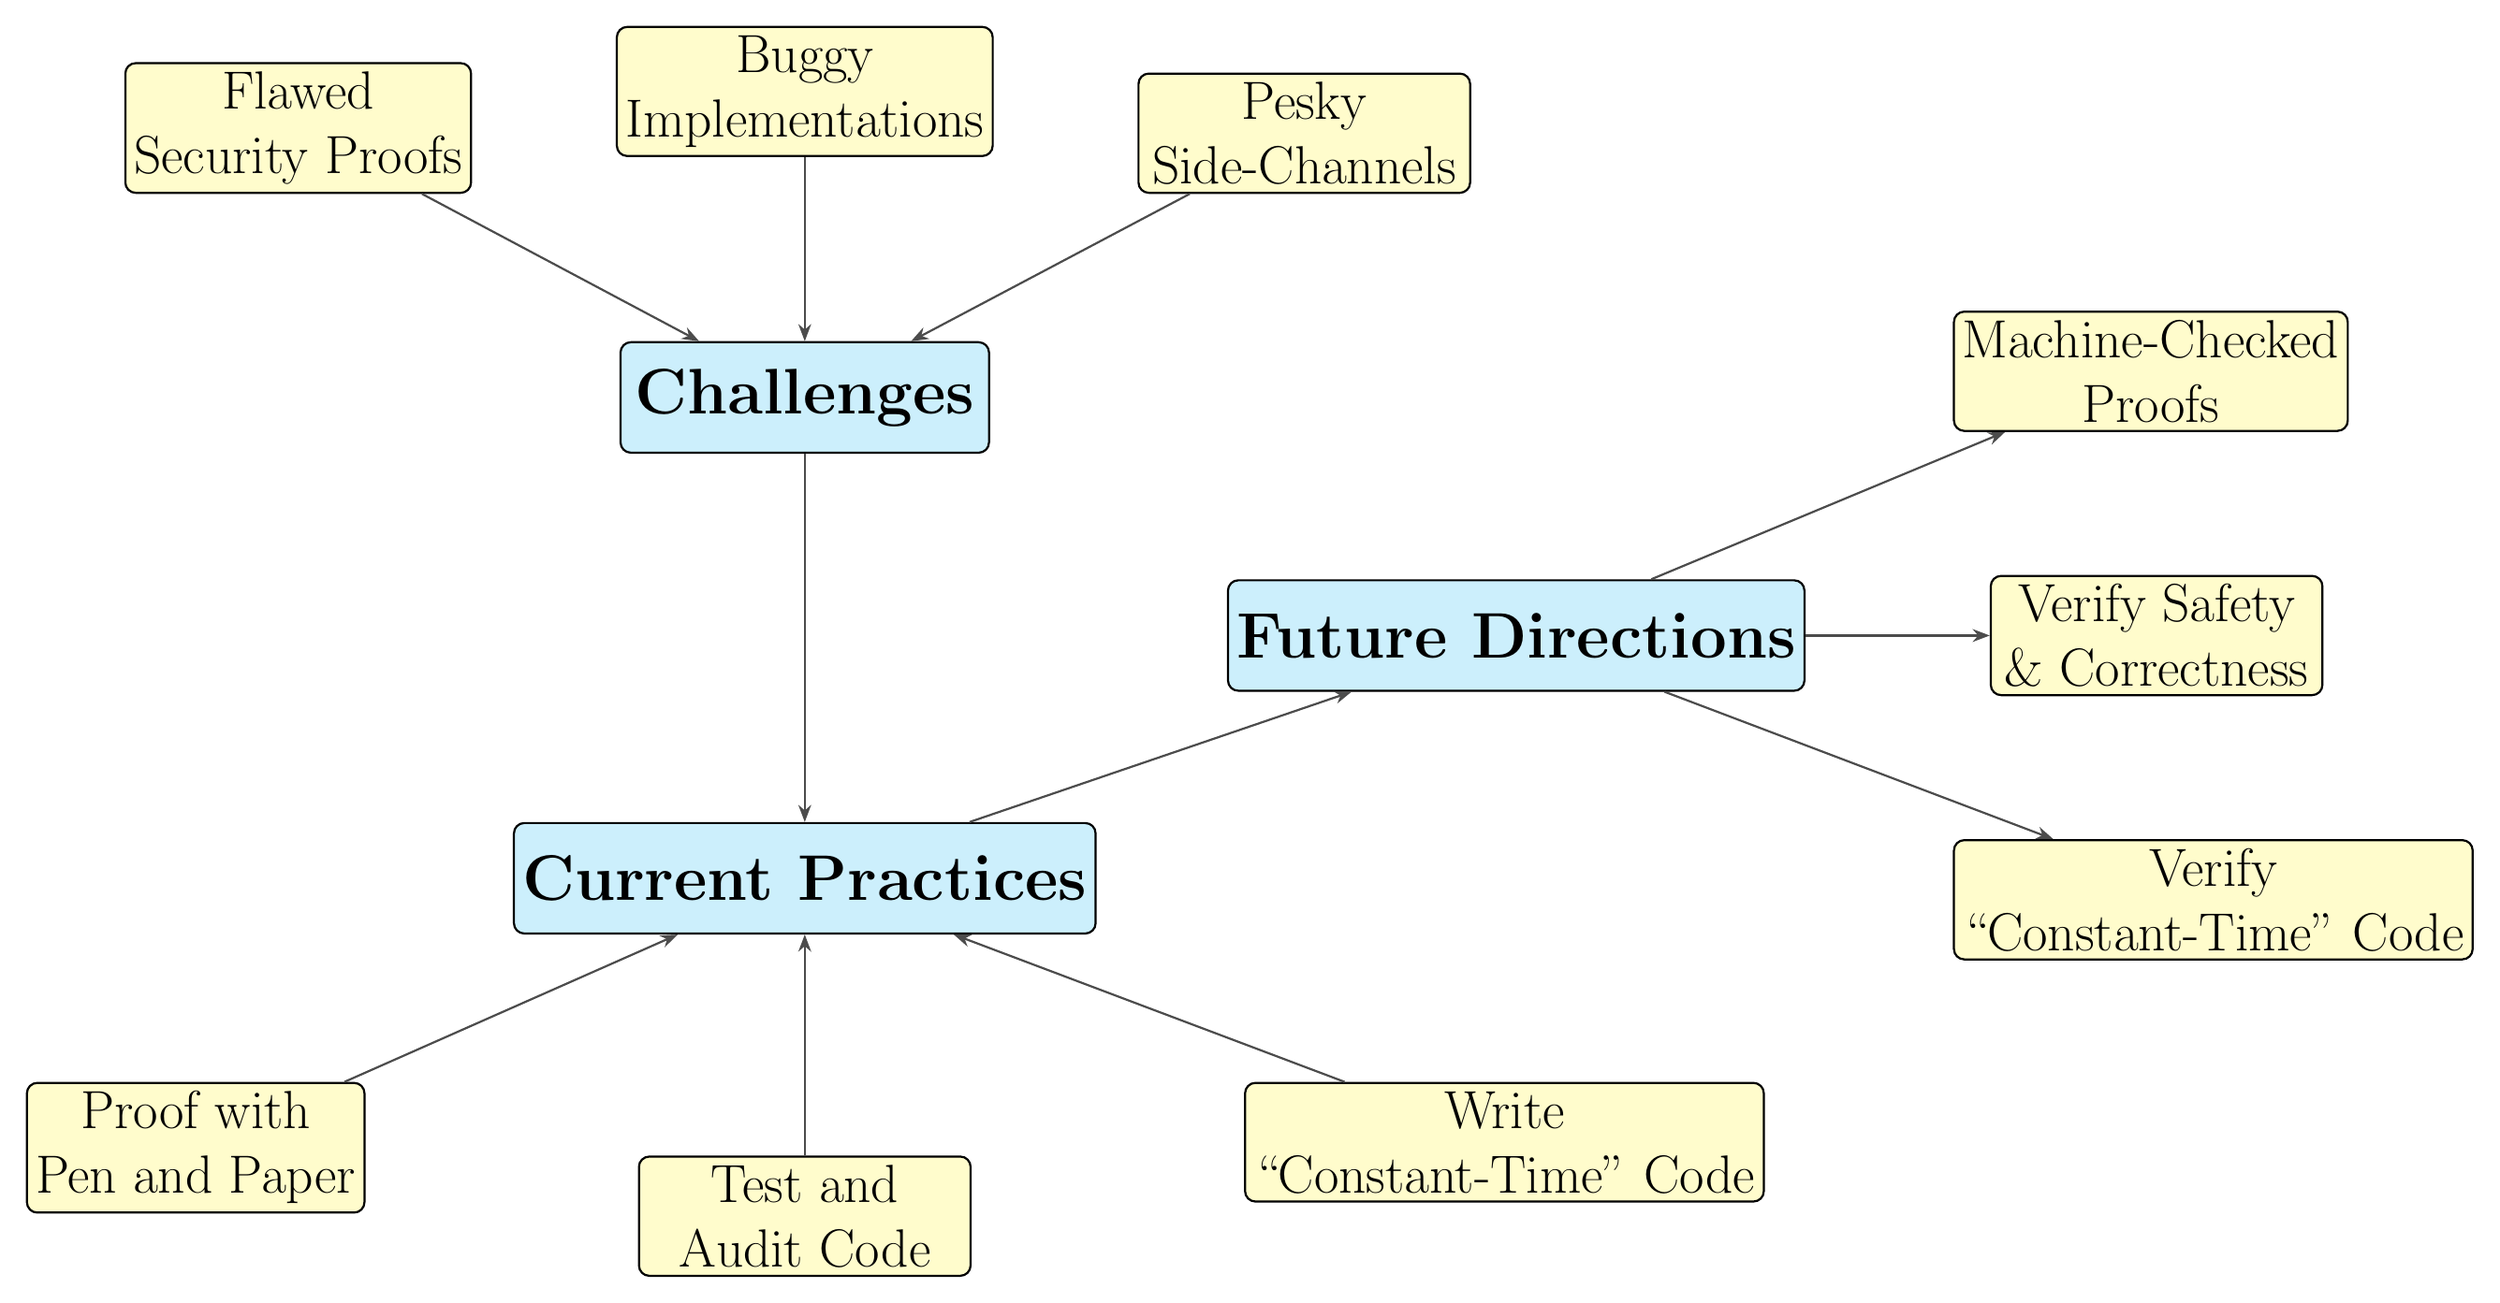
\begin{tikzpicture}[
mainconcept/.style={rectangle, rounded corners, minimum width=5cm, minimum height=1.5cm, text centered, draw=black, fill=cyan!20, font=\bfseries\Huge, thick},
subconcept/.style={rectangle, rounded corners, minimum width=4.5cm, minimum height=1.2cm, text centered, draw=black, fill=yellow!20, font=\huge, thick},
arrow/.style={thick,->,>=Stealth, draw=black!70},
% General Node Alignment
every node/.style={align=center}
]
% Main Nodes
\node (challenges) [mainconcept] {Challenges};
\node (practices) [mainconcept, below=5cm of challenges] {Current Practices};
\node (future) [mainconcept, above right=2.5cm of practices] {Future Directions};

% Subconcepts - Challenges
\node (flawed) [subconcept, above left=2cm and 2cm of challenges] {Flawed\\Security Proofs};
\node (buggy) [subconcept, above=2.5cm of challenges] {Buggy\\Implementations};
\node (side) [subconcept, above right=2cm and 2cm of challenges] {Pesky\\Side-Channels};

% Subconcepts - Current Practices
\node (proof) [subconcept, below left=2cm and 2cm of practices] {Proof with\\Pen and Paper};
\node (audit) [subconcept, below=3cm of practices] {Test and\\Audit Code};
\node (constant) [subconcept, below right=2cm and 2cm of practices] {Write\\``Constant-Time'' Code};

% Subconcepts - Future Directions
\node (machine) [subconcept, above right=2cm and 2cm of future] {Machine-Checked\\Proofs};
\node (verify) [subconcept, right=2.5cm of future] {Verify Safety\\\& Correctness};
\node (constantverify) [subconcept, below right=2cm and 2cm of future] {Verify\\``Constant-Time'' Code};

% Arrows - Challenges to Subconcepts
\draw [arrow] (flawed) -- (challenges);
\draw [arrow] (buggy) -- (challenges);
\draw [arrow] (side) -- (challenges);

% Arrows - Challenges to Practices
\draw [arrow] (challenges) -- (practices);

% Arrows - Current Practices to Subconcepts
\draw [arrow] (proof) -- (practices);
\draw [arrow] (audit) -- (practices);
\draw [arrow] (constant) -- (practices);

% Arrows - Practices to Future
\draw [arrow] (practices) -- (future);

% Arrows - Future Directions to Subconcepts
\draw [arrow] (future) -- (machine);
\draw [arrow] (future) -- (verify);
\draw [arrow] (future) -- (constantverify);
\end{tikzpicture}}
\end{center}

\newpage
\subsection{Design-level Security}


\newpage
\section{Specification for EasyCrypt}
\subsection{Type Expressions}
\EasyCrypt’s \textbf{type expressions} are derived from four fundamental constructs: \begin{enumerate}
	\item type variables, 
	\item type constructors (or named types), 
	\item function types, and 
	\item tuple (product) types. 
\end{enumerate} Type constructors may represent either built-in types or user-defined types, including record types and datatypes (variant types). Figure 0.0 outlines the syntax of these type expressions. Notably, all EasyCrypt types must be inhabited---that is, none can be empty.
\begin{figure}[h!]\centering
\begin{bnf}
$\tau,\sigma$ : ::=
| \texttt{tyvar} : type variable
| \texttt{\_} : anonymous type variable
| \texttt{($\tau$)} : parenthesized type
| \texttt{$\tau\to\sigma$} : function type
| \texttt{($\tau_1*\cdots*\tau_n$)} : tuple type
| \texttt{tyname} : named type
| \texttt{$\tau$ tyname} : applied type constructor
| \texttt{($\tau_1, \cdots, \tau_n$) tyname} : ibid.
;;
%$e$ : \textsf{Expr} ::=
%| $x$ : variable
%| $n$ : numeral
%| \texttt{$e$ + $e$} : addition
%| \texttt{$e$ * $e$} :
%multiplication
%| \texttt{$e$
%	\textasciicircum{} $e$} :
%concatenation
%| \texttt{len($e$)} : length
%| \texttt{let $x$ = $e_1$ in
%	$e_2$} : definition
\end{bnf}
\caption{\EasyCrypt’s type expressions}
\end{figure}
\begin{enumerate}
	\item \textit{A type variable}.
	
	These act like free variables for which a concrete type might later be substituted.
	\item \textit{An anonymous type variable}.  
	
	Serves as a placeholder when the specific identity of a type variable is unimportant or omitted.
	\item \textit{A parenthesized type}, used purely for grouping.  
	
	E.g. \((\tau)\) is the same as \(\tau\), but parentheses may clarify precedence.
	
	\item \textit{A function type}.
	  
	In standard category-theoretic terms, this is the type \(\tau \to \sigma\) of morphisms from \(\tau\) to \(\sigma\). It is also akin to the set of total functions from the set (or type) \(\tau\) to the set (type) \(\sigma\).
	
	\item \textit{A tuple type}.
	  
	Interpreted as a \textit{product type}, i.e., \(\tau_1 \times \cdots \times \tau_n\).  
	
	\item \textit{A named type}.  
	
	This might be a base type (like \(\texttt{int}, \texttt{bool}\), or \(\texttt{real}\)) or another type name declared in a theory. Algebraically, one can think of these as \textit{atomic} or \textit{defined} types.
	
	\item \textit{An applied type constructor} in unary form.  
	
	For instance, if \(\mathtt{tyname}\) is a unary type constructor \(T\), then \(\tau\ \mathtt{tyname}\) is the \textit{instantiation} of \(T\) at the type \(\tau\).  
	
%	In functional languages, you might see something like `\texttt{list a}' or `option β`. This syntax is similar: one has a constructor \(T\) that is parameterized by the type variable \(\tau\).
	
	\item \textit{An applied type constructor} taking \(n\) parameters.  
	
	If \(\mathtt{tyname}\) is an \(n\)-ary constructor (like a generic container type \(\mathrm{Map}(\cdot,\cdot)\) expecting two type parameters), then \(\bigl(\tau_1,\ldots,\tau_n\bigl)\ \mathtt{tyname}\) is its instantiation at types \(\tau_1,\ldots,\tau_n\).
	
	Mathematically, think of this as \(T(\tau_1,\dots,\tau_n)\), where \(T\) is an \(n\)-ary functor on types.
\end{enumerate}


%\begin{center}
%	\begin{bnf}
%		$\tau$ : \textsf{Type} ::=
%		| \texttt{num} : numbers
%		| \texttt{str} : strings
%		;;
%		$e$ : \textsf{Expr} ::=
%		| $x$ : variable
%		| $n$ : numeral
%		| \texttt{$e$ + $e$} : addition
%		| \texttt{$e$ * $e$} :
%		multiplication
%		| \texttt{$e$
%			\textasciicircum{} $e$} :
%		concatenation
%		| \texttt{len($e$)} : length
%		| \texttt{let $x$ = $e_1$ in
%			$e_2$} : definition
%	\end{bnf}
%\end{center}
%
%\begin{bnf}[
%	colspec = {llcll},
%	column{1} = {font = \sffamily},
%	column{2} = {mode = dmath},
%	column{4} = {font = \ttfamily},
%	]
%	\tau : Type ::=
%	| num : numbers
%	| str : strings
%	;;
%	e : Expr ::=
%	| $x$ : variable
%	| $n$ : numeral
%	| $e$ + $e$ : addition
%	| $e$ * $e$ : multiplication
%	| $e$ \textasciicircum{} $e$ : concatenation
%	| len($e$) : length
%	| let $x$ = $e_1$ in $e_2$ : definition
%\end{bnf}
%\section{Introduction to EasyCrypt}
%\subsection{EasyCrypt Environment}
\EasyCrypt is developed in \OCaml and integrates several external tools and libraries. The key components that will be most relevant to our work are as follows:

\begin{enumerate}
	\item \textbf{\Emacs and \ProofGeneral}
	
	\Emacs, a widely-used open-source text editor, serves as the foundation for \ProofGeneral, a generic interface designed for proof assistants. Together, they provide the primary front-end environment for interacting with \EasyCrypt. Typically, proofs in \EasyCrypt are constructed interactively using the \Emacs + \ProofGeneral setup.
	\item \textbf{External Provers and \WhyThree}
	
	Satisfiability Modulo Theory (\SMT) solvers, often referred to as external provers, are powerful tools designed to determine the satisfiability of formulas under a set of constraints. \EasyCrypt integrates with several prominent \SMT solvers, including \AltErgo, \ZThree, and \CVCFour, all of which are managed through the \WhyThree platform.
	
	These external provers handle much of the intricate, low-level work involved in proving mathematical results. As we will demonstrate, they significantly streamline the proving process by automating many of the more arduous and repetitive tasks.
\end{enumerate}

\subsection{A Guide to Installing EasyCrypt (v250121)}
The official \EasyCrypt installation instructions are available on the \hyperref{https://github.com/EasyCrypt/easycrypt}{github}{ec}{EasyCrypt GitHub} repository. We provides a summary of these instructions, with a particular focus on their integration with the \hyperref{https://www.gnu.org/software/emacs/}{site}{emacs}{Emacs} text editor.\par
\EasyCrypt can operate in batch mode from the shell (command line) to check individual \texttt{.ec} files. However, interactive proof construction is conducted within \Emacs, utilizing the generic interface \ProofGeneral, which acts as a mediator between \Emacs and \EasyCrypt, the latter running as a sub-process of Emacs.

These instructions are aligned with the following software versions:
\begin{itemize}
	\item \OCaml compiler version 5.1.1
	\item \WhyThree version 1.7.2
	\item \AltErgo version 2.5.2
\end{itemize}
\EasyCrypt is implemented in \OCaml. \WhyThree serves as the interface to \SMT solvers used by \EasyCrypt, and \AltErgo is one of the \SMT solvers required for its operation.

\subsubsection*{Step 1. Installing Emacs}
\begin{lstlisting}[style=normal]
@:~$ sudo apt-get install emacs
@:~$ sudo apt-get update
\end{lstlisting}

\subsubsection*{Step 2. Installing EasyCrypt on Linux}
\begin{itemize}
	\item \hl{\texttt{opam init}} : creates .opam sub-directory of your home directory
	\item \hl{\texttt{eval \$(opam env)}} : updates environment variables in current shell
	\item \hl{\texttt{opam switch create 5.1.1}} : say which version of \OCaml compiler to build
\end{itemize}
\begin{lstlisting}[style=normal]
@:~$ sudo apt-get install autoconf

@:~$ opam init
@:~$ eval $(opam env)

@:~$ opam switch create 5.1.1
@:~$ eval $(opam env)

@:~$ opam pin -yn add easycrypt https://github.com/EasyCrypt/easycrypt.git
@:~$ opam install --deps-only easycrypt
@:~$ eval $(opam env)

@:~$ opam pin why3 1.8.0
@:~$ opam pin alt-ergo 2.5.2
\end{lstlisting}

There are binaries at this URL \url{https://github.com/Z3Prover/z3/releases/tag/z3-4.12.4}. If you need to build it from source, there are source archives available, too. Assuming you have the binary distribution, put the whole directory somewhere, and update your shell's startup script to add its bin directory to the PATH environment variable. Run which z3 while not in the Z3 bin directory to verify that you have set up PATH correctly.
\[
\texttt{export PATH="/home/username/z3-4.12.4-x64-glibc-2.35/bin:\$PATH"}
\]
\begin{lstlisting}[style=normal]
@:~$ which z3
/home/username/z3-4.12.4-x64-glibc-2.35/bin/z3
\end{lstlisting}

\begin{lstlisting}[style=normal]
@:~$ opam install easycrypt
@:~$ eval $(opam env)

@:~$ which easycrypt
/home/username/.opam/5.1.1/bin/easycrypt

@:~$ easycrypt why3config
Executing: why3 config detect -C /home/username/.config/easycrypt/why3.conf
warning: cannot read config file /home/username/.config/easycrypt/why3.conf:
/home/hacker-code-j/.config/easycrypt/why3.conf: No such file or directory
Found prover Alt-Ergo version 2.5.2, OK.
Found prover Alt-Ergo version 2.5.2 (alternative: counterexamples)
Found prover CVC4 version 1.8 (alternative: strings+counterexamples)
Found prover CVC4 version 1.8 (alternative: strings)
Found prover CVC4 version 1.8 (alternative: counterexamples)
Found prover CVC4 version 1.8, OK.
Found prover Z3 version 4.12.4 (alternative: counterexamples)
Found prover Z3 version 4.12.4, OK.
Found prover Z3 version 4.12.4 (alternative: noBV)
9 prover(s) added
Save config to /home/username/.config/easycrypt/why3.conf
\end{lstlisting}


\begin{lstlisting}[style=normal]
@:~$ touch .emacs
@:~$ emadcs .emacs
\end{lstlisting}
\begin{lstlisting}[style=normal]
(require 'package)
(add-to-list 'package-archives '("melpa" . "https://melpa.org/packages/") t)
(package-initialize)
\end{lstlisting}


\newpage
\subsection{\INDRoR game}
We model a game to demonstrate that a cryptographic protocol ensures the property of ciphertexts being indistinguishable from random. This property, commonly abbreviated as \textsf{IND-RoR} (Indistinguishability -- Real or Random), is one of the foundational security guarantees expected from cryptographic systems. At its core, the concept asserts that if an adversary cannot differentiate between an encrypted message and an encryption of random data, they are unable to extract any meaningful information from intercepted ciphertexts beyond what would be possible by pure chance. This notion forms the basis for considering such a system secure.\par
To formalize this mathematically, we consider a cryptographic protocol, denoted as $\Pi$, which includes an encryption function, $\enc$, and a decryption function, $\dec$, both known to the challengers. The adversary is granted access to the output of $\enc$. For simplicity, the specific details of these functions are not addressed in this model.\par
The \INDRoR game for the protocol $\Pi$ is then defined as follows:
\begin{enumerate}
	\item Select $b\in\set{0,1}$ uniformly at random.
	\item If $b=0$, the challengers encrypt a real message $m_{\text{real}}$, using the encryption function $\enc$, producing $c_0=\enc(m_{\text{real}})$.
	\item If $b=1$, the challengers encrypt a random bit-string $m_{\text{random}}$ using $\enc$, resulting in $c_1=\enc(m_{\text{random}})$.
	\item Depending on the value of $b$, the challengers send either $c_0$ (if $b=0$) or $c_1$ (if $b=1$) to the adversary.
	\item The adversary is then allowed to perform computations on the received ciphertext and is expected to produce an output $b_{\text{adv}}$, representing their guess of the value of $b$.
	\item The adversary is considered to have won the game if they can correctly distinguish between the real and random ciphertexts with a non-negligible advantage over random guessing. Mathematically, the adversary wins if: \[
	\Pr[b_{\text{adv}}=b]=\frac{1}{2}+\varepsilon,\ \text{where $\varepsilon$ is non-negligible}
	\]
\end{enumerate}
If we can establish a proof demonstrating that $\Pr[b_{\text{adv}}=b]=\frac{1}{2}+\varepsilon$ where $\varepsilon$ is negligible irrespective of the adversary's actions, we can assert that the protocol is secure under the \INDRoR framework.\par
Game-based proofs, such as this one, are a cornerstone of establishing security properties for most cryptographic protocols. Although our example has been significantly simplified, it can already be effectively modeled using \EasyCrypt.

\subsection{Modeling the \INDRoR game with EasyCrypt}
We now proceed to outline an \EasyCrypt proof sketch for the game defined earlier. Every \EasyCrypt proof typically involves the following key steps:
\begin{enumerate}[\bfseries\text{Step.} 1]
	\item \textbf{[Defining the objects]}
	
	To begin, we need to establish the working context. \EasyCrypt provides several predefined \emph{types}, \emph{operators}, and \emph{functions}, including integers, real numbers, and more. To utilize these, we first load (\ecinline{require}) and import (\ecinline{import}) the relevant theories into the current environment. These theories, contained within theory files, provide the necessary definitions and constructs for our work.
	
	In this example, we will require the \ecinline{Real}, \ecinline{Bool}, and \ecinline{DBool} theory files. The \ecinline{Real} and \ecinline{Bool} theories allow us to work with real numbers and boolean types, respectively, while the \ecinline{DBool} theory (boolean distribution) enables us to sample boolean values randomly. Theories can be imported as follows:\\
	\eccode[caption={Importing theory files}]{listings/importing_theories.ec}
	
	It is worth noting that in \EasyCrypt, statements are terminated with a period (\ecinline{.}).
	
	Beyond the predefined types, we may need custom data types and operations to fit specific use cases. \EasyCrypt enables this through the \ecinline{type} and \ecinline{op} keywords. For this example, we define two custom types: \ecinline{msg} for messages and \ecinline{cip} for ciphertexts. We then define the following operations:
	\begin{itemize}
		\item \ecinline{enc: msg -> cip}, which maps a message to a ciphertext.
		\item \ecinline{dec: cip -> msg}, which maps a ciphertext back to its original message.
	\end{itemize}
	Additionally, we define a function \ecinline{comp: cip -> bool}, which models the adversary performing computations on a ciphertext and returning a boolean value as a result.
	\newpage
	\eccode[caption={Defining types and ops}]{listings/types_and_ops.ec}
	\begin{lstlisting}[style=normal]
+ added type: `msg'
+ added type: `cip'
+ added operator enc : msg -> cip
+ added operator dec: cip -> msg
+ added operator comp: cip -> bool
	\end{lstlisting}
	It is important to note that these definitions are purely abstract; we have not specified the details of the types or functions. One of the advantages of \EasyCrypt is its ability to work effectively with such abstract types and operations, allowing significant progress even without concrete implementations.
	
	Next, we define custom module types and modules. In \EasyCrypt, a \textbf{module type} serves as a blueprint, while a \textbf{module} represents a concrete instantiation of a module type. For those familiar with object-oriented programming, this is analogous to interfaces and their implementing classes. Module types act as interfaces, and modules are similar to singleton classes that conform to these interfaces.

	In our example, the challengers need the ability to encrypt and decrypt messages. To model this behavior, we define a module type called \ecinline{Challenger}, which specifies the procedures encrypt and decrypt. Since a module type is just a blueprint, we need to instantiate it to work with it concretely. We accomplish this by creating a module \ecinline{C} of type \ecinline{Challenger}, implementing the required \ecinline{encrypt} and \ecinline{decrypt} procedures. This is done as follows:\\
	\eccode[caption={Defining module types and modules}]{listings/module_type_and_modules.ec}
\end{enumerate}


\newpage
\subsection{Logics in EasyCrypts}
Having established an understanding of the overarching structure and capabilities of \EasyCrypt, we now turn our attention to the details.

\EasyCrypt provides the flexibility to work with a variety of mathematical objects and results of differing types. To manage these various results effectively, \EasyCrypt incorporates the following logical frameworks:
\begin{table}[h!]\centering\setstretch{1.25}
\begin{tabularx}{\textwidth}{>{\centering\arraybackslash}p{.1\textwidth}||>{\raggedright\arraybackslash}p{.495\textwidth}|>{\raggedright\arraybackslash}p{.345\textwidth}}
\toprule[1.2pt]
& \textbf{Ambient Logic} & \textbf{Hoare Logic} \\ \midrule
\textbf{Scope} & Overall reasoning framework (includes probabilities, expectations, etc.). & Specific tool for reasoning about program correctness.\\ \hline
\textbf{Roll in \EC} & Provides the probabilistic foundation, equational reasoning, and constructs for games. & Used to reason about correctness of cryptographic programs \\ \hline
\textbf{Focus} & General framework for proofs and logical reasoning. & Verifying how program states evolve.\\ \bottomrule[1.2pt]
\end{tabularx}
\end{table}
\begin{enumerate}
	\item \textbf{Ambient logic}:
	
	This is a higher-order logic framework that enables reasoning about proof objects and terms.
	\item \textbf{Hoare logic and its variants}:
	\begin{enumerate}
		\item \textbf{Hoare Logic (HL)}: A foundational logic that facilitates reasoning about individual programs or sets of instructions.
		\item \textbf{Relational Hoare Logic (RHL)}: Extends Hoare Logic to allow reasoning about pairs of programs.
		\item \textbf{Probabilistic Hoare Logic (pHL)}: Designed to handle programs exhibiting probabilistic behavior by incorporating probabilistic elements into Hoare Logic. \EasyCrypt supports reasoning about such probabilistic programs.
		\item \textbf{Probabilistic Relational Hoare Logic (pRHL)}: An extension of RHL that enables reasoning about pairs of programs that involve probabilistic behavior.
	\end{enumerate}
\end{enumerate}
Using these logical frameworks, \EasyCrypt provides the capability to verify the security properties of cryptographic protocols. Most cryptographic proofs are game-based, requiring the ability to reason about pairs of programs, as illustrated in the IND-RoR example. This necessity underpins the importance of RHL and pRHL in cryptographic proofs.

In addition to its internal logical frameworks, \EasyCrypt leverages external SMT solvers to automate various aspects of the proving process. SMT solvers are tools that determine whether a mathematical formula is satisfiable under a given set of constraints.

In the following chapters, we will explore how to work with these logical frameworks and integrate external SMT solvers into the proof development process.


\newpage
\section{EasyCrypt's Ambient Logic I}
The ambient logic in \EasyCrypt serves as the foundation for all proof scripts. To gain a deeper understanding of its functionality, we will explore several examples. 
%All the examples discussed in this section are also included in the `\texttt{ambient-logic.ec}' file. While it is strongly recommended to work through this file using \EasyCrypt in the \ProofGeneral + \Emacs environment, reading through this chapter alone will provide a solid understanding of ambient logic and the associated proof tactics introduced here.

As demonstrated in the earlier motivating example, formal proofs are constructed as a sequence of proof tactics. Up to this point, we have only encountered the admit tactic. In this chapter, we will expand on this by introducing additional basic tactics and applying them to simple mathematical properties of integers.

\subsection{Basic Tactics and Theorem Proving}
\EasyCrypt features a typed expression language, meaning every declared entity must either have an explicitly defined type or a type that can be inferred from the context. As previously noted, \EasyCrypt provides basic built-in data types, which can be accessed by importing the relevant theories into the current environment. For this particular file, we will work with the `\ecinline{Int}' theory file. Additionally, to enable \EasyCrypt to display all the proof goals during our work, we use a directive known as a pragma.\\
\eccode[linerange={1-2}, caption={Imports and pragma}]{listings/ambient-logic-tatics.ec}

Typically, the initial steps in \EasyCrypt scripts involve importing the required theories and setting the appropriate pragmas. Before delving into cryptography, it is essential to understand how to guide \EasyCrypt in modifying proof goals and making progress. This process is facilitated by the use of tactics. In general, the proofs for lemmas in \EasyCrypt follow a structured approach, as illustrated below:\\
\eccode[caption={Proof script form}]{listings/proof_script_form.ec}

\subsubsection{Tactic: \ecinline{trivial}}
We begin by exploring some basic properties of integers and demonstrating how a few key tactics operate in \EasyCrypt.

Reflexivity, the property that any integer is equal to itself, can be expressed mathematically as: \[
\forall n\in\Z,\ n=n.
\] In EasyCrypt, this property can be stated as a lemma and proved as follows:\\
\eccode[linerange={4-7}, caption={Using the \ecinline{trivial} tactic}]{listings/ambient-logic-tatics.ec}

Once the lemma is declared and evaluated, \EasyCrypt populates the goal pane with the statement that needs to be proved. For this lemma, the goal pane displays the reflexivity property.\\
%caption={Goal upon evaluating `\ecinline{int_refl}'}
\begin{lstlisting}[style=normal]
Current goal
Type variables: <none>
----------------------------
forall (n : int), n = n
\end{lstlisting}

The proof script begins with the \ecinline{proof} keyword, after which \EasyCrypt expects the application of tactics to close the goal. In this case, we use the trivial tactic to prove the lemma \ecinline{int_refl}. Upon applying \ecinline{trivial}, the goal pane is cleared since this tactic successfully resolves the goal. When all goals are resolved, the proof can be concluded with \ecinline{qed}. This saves the lemma for future use, and \EasyCrypt provides confirmation in the response pane as shown:\\
\begin{lstlisting}[style=normal]
+ added lemma: `int_refl'
\end{lstlisting}
The \ecinline{trivial} tactic attempts to solve the goal by applying a variety of internal tactics. While it may sometimes be unclear when it will succeed, the advantage of \ecinline{trivial} is that it never fails—it either resolves the goal or leaves it unchanged. This makes it a safe and effective tactic to apply without any risk of disruption.

\newpage
\subsubsection{Tactic: \ecinline{apply}}
Once the lemma \ecinline{int_refl} is proved, \EasyCrypt stores it and allows us to use it to prove other lemmas. This is accomplished using the \ecinline{apply} tactic. For example:\\
\eccode[linerange={9-12}, caption={Using the \ecinline{apply} tactic}]{listings/ambient-logic-tatics.ec}
The \ecinline{apply} tactic works by attempting to match the conclusion of the provided proof term with the goal’s conclusion. If a match is found, the goal is replaced by the subgoals of the proof term.

In this case, \EasyCrypt matches \ecinline{int_refl} with the goal’s conclusion, verifies the match, and replaces the goal with the subgoals required for \ecinline{int_refl}. Since there are no additional subgoals to prove for \ecinline{int_refl}, the proof is concluded successfully.

\EasyCrypt also includes a library of predefined lemmas and axioms that can be used to facilitate proofs. For example, \ecinline{addzC} and \ecinline{addzA} are axioms related to the commutativity and associativity of integer addition, respectively. We can inspect these predefined lemmas and axioms using the \ecinline{print} command. For instance, running \ecinline{print addzC} and \ecinline{print addzA} prompts \EasyCrypt to display the following:\\
\begin{lstlisting}[style=easycrypt]
axiom nosmt addzC: forall (x y : int), x + y = y + x.
\end{lstlisting}
\begin{lstlisting}[style=easycrypt]
axiom nosmt addzA: forall (x y z : int), x + (y + z) = x + y + z.
\end{lstlisting}

\newpage
\subsubsection{Tactic: \ecinline{simplify}}
In proofs, it is common for tactics to produce goals that can be simplified. To handle such cases, we use the \ecinline{simplify} tactic, which reduces the goal to its normal form using principles of lambda calculus. While the underlying mechanics of this process need not concern us, it is crucial to understand that \EasyCrypt simplifies goals whenever possible, provided it has sufficient knowledge to do so. If the goal is already in normal form, the simplify tactic leaves it unchanged.

For example, the following illustration demonstrates the use of the \ecinline{simplify} tactic:\\
\eccode[linerange={14-24}, caption={Using the \ecinline{simplify} tactic}]{listings/ambient-logic-tatics.ec}
\begin{center}
\begin{minipage}{.25\textwidth}
\begin{lstlisting}[style=normal]
Current goal
Type variables: <none>

x: int
----------------------
x + 2 * 3 = 6 + x
\end{lstlisting}
\end{minipage}\hfill$\xrightarrow{\color{blue}\texttt{\bfseries simplify}}$\hfill
\begin{minipage}{.25\textwidth}
\begin{lstlisting}[style=normal]
Current goal
Type variables: <none>

x: int
----------------------
x + 6 = 6 + x
\end{lstlisting}
\end{minipage}\hfill$\xrightarrow{\color{blue}\texttt{\bfseries simplify}}$\hfill
\begin{minipage}{.25\textwidth}
\begin{lstlisting}[style=normal]
Current goal
Type variables: <none>

x: int
----------------------
x + 6 = 6 + x
\end{lstlisting}
\end{minipage}
\end{center}

\newpage
\subsubsection{Tactics: \ecinline{move}, \ecinline{rewrite}, \ecinline{assumption}}
Until now, we have worked with lemmas that did not involve any assumptions, apart from specifying variable types. However, in most cases, we will need to incorporate assumptions about variables into our proofs. These assumptions are treated as given and are introduced into the context using the \ecinline{move =>} command, followed by the desired name for the assumption.

When such assumptions appear as goals, rather than explicitly applying them, we can use the \ecinline{assumption} tactic to discharge the goal directly. This tactic instructs \EasyCrypt to automatically search for assumptions in the context that match the goal and apply them.

Consider the following example, where we use the axiom \ecinline{addz_gt0}, which is stated as follows:\\
\begin{lstlisting}[style=easycrypt]
axiom nosmt addz_gt0: forall (x y : int), 0 < x => 0 < y => 0 < x + y.
\end{lstlisting}
Using this result, we construct the following proof script:\\
\eccode[linerange={26-40}, caption={Proof for \ecinline{x_pos}}]{listings/ambient-logic-tatics.ec}
In this proof, the \ecinline{rewrite} tactic modifies the goal by replacing the current expression with a specified pattern. For example, in this case, the goal 
\ecinline{0 < x + 1} is rewritten using the pattern from \ecinline{addz_gt0}, resulting in subgoals that require proving the assumptions \ecinline{0 < x} and \ecinline{0 < 1}.
\begin{center}
\hfill\begin{minipage}{.25\textwidth}
\begin{lstlisting}[style=normal]
Current goal
Type variables: <none>

x: int
----------------------
0 < x => 0 < x + 1	
\end{lstlisting}
\end{minipage}\hfill$\xrightarrow[\texttt{x\_ge0}]{\texttt{\textcolor{blue}{\bfseries move} =>}}$\hfill
\begin{minipage}{.25\textwidth}
\begin{lstlisting}[style=normal]
Current goal
Type variables: <none>

x: int
x_ge0: 0 < x
----------------------
0 < x + 1	
\end{lstlisting}
\end{minipage}
\end{center}
\begin{center}
\hfill$\xrightarrow[\texttt{addz\_gt0}]{\texttt{\textcolor{blue}{\bfseries rewrite}}}$\hfill
\begin{minipage}{.35\textwidth}
\begin{lstlisting}[style=normal]
Current goal (remaining: 2)
Type variables: <none>

x: int
x_ge0: 0 < x
----------------------
0 < x


	Goal #2	
	----------------------
	0 < 1
\end{lstlisting}
\end{minipage}\hfill$\xrightarrow{\texttt{\textcolor{red}{\bfseries assumption}}}$\hfill
\begin{minipage}{.25\textwidth}
\begin{lstlisting}[style=normal]
Current goal
Type variables: <none>

x: int
x_ge0: 0 < x
----------------------
0 < 1	
\end{lstlisting}
\end{minipage}
\end{center}
Sometimes, a lemma or axiom may be rewritten to the goal, but the left-hand side (LHS) and right-hand side (RHS) of the expression might be flipped. To address this, we can rewrite the lemma or axiom in reverse by prefixing the lemma with a `\ecinline{-}' symbol. This approach enables rewriting the sides as follows:\\
\eccode[linerange={42-47}, caption={Rewriting in reverse}]{listings/ambient-logic-tatics.ec}
These tactics constitute the foundational tools for theorem proving in \EasyCrypt, particularly when working at the level of ambient logic.

It is worth noting that these tactics, while simple, include a variety of options and intricacies. For instance, the \ecinline{move =>} tactic supports many introduction patterns, and the keyword move can be substituted with other tactics depending on the context. Expanding on these introduction patterns with clear examples would be a valuable addition to this discussion on basic tactics.
\newpage
\subsubsection{Commands: \ecinline{search} and \ecinline{print}}
When working with theorems, it is often necessary to search through results already available in the environment. While we have encountered a few examples of printing in the content covered so far, it is useful to take a more detailed look at this aspect of \EasyCrypt, as it is a feature we frequently rely on.

The \ecinline{print} command outputs the requested information in the response pane. This command can be used to print various elements, such as types, modules, operations, and lemmas, by using the print keyword. For example:\\
\eccode[linerange={49-54}, caption={Using the \ecinline{print} command}]{listings/ambient-logic-tatics.ec}

Keywords serve as qualifiers and filters to refine the results. However, it is not mandatory to use qualifiers; printing without them will display broader results, while qualifiers help narrow the scope of the output.

The \ecinline{search} command allows us to locate axioms and lemmas involving specific operators. This command takes arguments enclosed in braces to perform the search:
\begin{enumerate}
	\item \texttt{[]} - Square brackets for unary operators
	\item \texttt{()} - Round brackets for binary operators
	\item Names of operators
	\item Combination of these separated by a space
\end{enumerate}

\eccode[linerange={56-65}, caption={Using the \ecinline{search} command}]{listings/ambient-logic-tatics.ec}

\newpage
\subsubsection{External solvers: \ecinline{smt}}
It is essential to understand that \EasyCrypt (\EC) was primarily designed to handle cryptographic properties and more complex constructs. While it is possible to prove general mathematical theorems and claims in \EC, the process can be cumbersome. To address the challenge of low-level logic and tactics, \EC integrates with powerful automated tools through the \ecinline{smt} tactic.

When the \ecinline{smt} tactic is invoked, \EC sends the current goal and its context to external \SMT solvers, such as \ZThree and \AltErgo, which are pre-configured for use with \EC. If the \SMT solver can resolve the goal, the \ecinline{smt} tactic automatically discharges the specific subgoal. However, if the solver fails to find a solution, the proof remains incomplete, and the responsibility of resolving the goal falls back on the user.

For instance, consider the following results: \begin{align*}
\forall x\in\R,\ \forall a,b\in\Z,\ &x^{a\cdot b}=(x^a)^b,\\
\forall x\in\R,\ \forall a,b\in\Z,\ &x\neq0\implies x^a\cdot x^b=x^{a+b}.
\end{align*}
These can be proved in EC using the following script:\\
\eccode[linerange={66-83}, caption={Manual proof for \ecinline{exp_prod} and \ecinline{exp_prod2}}]{listings/ambient-logic-tatics.ec}
Alternatively, the proof can be simplified to:\\
\eccode[linerange={85-93}, caption={Using \ecinline{smt} to prove \ecinline{exp_prod_smt} and \ecinline{exp_prod2_smt}}]{listings/ambient-logic-tatics.ec}
The key takeaway is that we will depend heavily on external solvers to handle a significant portion of the computational workload, particularly for results involving low-level mathematics.

This chapter concludes with an overview of ambient logic. We covered fundamental tactics such as \ecinline{apply}, \ecinline{simplify}, \ecinline{move}, and \ecinline{rewrite}, along with the usage of \ecinline{search} and \ecinline{print} commands. Additionally, we explored how to work with external solvers to streamline the proving process. In subsequent chapters, we will introduce more advanced tactics and techniques to expand on this foundation.
%\newpage
\subsection{Ambient Logic's Exercies: Level 1}
\begin{enumerate}[\textbf{[}\bfseries1\textbf{]}]
\item 
\end{enumerate}
%\begin{enumerate}[\textbf{[}\bfseries1\textbf{]}]
%\item The `\ecinline{admit}' tactic resolves the current goal by assuming its truth without proof. Replace the `\ecinline{admit}' tactic in the following lemma and prove it. (\textcolor{red}{\bfseries Do not use `\ecinline{smt}'.})\\
%\begin{lstlisting}[style=easycrypt]
%lemma x_minus_equal (x: int): x - 10 = x - 9 - 1.
%proof.
%admit.
%qed.
%\end{lstlisting}
%\begin{proof}[\sol]
%\ \color{gray!20}
%\begin{lstlisting}[style=normal]
%	proof.
%	trivial.
%	qed.
%\end{lstlisting}
%\end{proof}
%\item Apply the `\ecinline{split}' tactic to divide the disjunction into two separate goals. Then, utilize the earlier defined axioms to resolve these goals. (\textcolor{red}{\bfseries Do not use `\ecinline{smt}'.})\\
%\begin{lstlisting}[style=easycrypt]
%lemma int_assoc_comm (x y z: int): x + (y + z) = (x + y) + z /\ x + y = y + x.
%proof.
%admit.
%qed.
%\end{lstlisting}
%\begin{proof}[\sol]
%\ \color{gray!20}
%\begin{lstlisting}[style=normal]
%	proof.
%	split.
%	(* Goal 1: x + (y + z) = x + y + z *)
%	rewrite addzA.
%	trivial.
%	(* Goal 2: x + y = y + x *)
%	rewrite addzC.
%	trivial.
%	qed.
%\end{lstlisting}
%\end{proof}
%\item \textcolor{red}{\bfseries Do not use `\ecinline{smt}'.}\\
%\begin{lstlisting}[style=easycrypt]
%require import AllCore.  (* for `%r' *)
%require import RealExp.  (* for `ln' *)
%
%lemma ln_prod (x y: real): 0%r < x  => 0%r < y => ln (x*y) = ln x + ln y.
%proof.
%search (ln) (+).
%admit.
%qed.
%\end{lstlisting}
%\begin{proof}[\sol]
%\ \color{gray!20}
%\begin{lstlisting}[style=normal]
%	proof.
%	search (ln) (+).
%	move => H1 H2.
%	by apply lnM.
%	qed.
%\end{lstlisting}
%\end{proof}
%% Problem 4
%\item \textcolor{red}{\bfseries Do not use `\ecinline{smt}'.}\\
%\begin{lstlisting}[style=easycrypt]
%require import AllCore.
%require import IntDiv.
%
%lemma mod_add (x y z: int): (x %% z + y %% z) %% z = (x + y) %% z.
%proof.
%admit.
%qed.
%\end{lstlisting}
%\begin{proof}[\sol]
%\ \color{gray!20}
%\begin{lstlisting}[style=normal]
%	proof.
%	print IntDiv.
%	print modzDm.
%	by apply modzDm.
%	qed.
%\end{lstlisting}
%\end{proof}
%\end{enumerate}
%\newpage
\subsection{Ambient Logic's Exercies: Level 2}

\begin{enumerate}[\textbf{[}\bfseries1\textbf{]}]
\item We want to prove that \( \neg (a \lor b) \implies \neg a \land \neg b \).
\[
\infer[\neg \text{Introduction}]{\neg a \land \neg b}{\neg (a \lor b)}
\]
\begin{proof}[\normalfont\text{[Part I]}]
\( \neg (a \lor b) \implies (\neg a \land \neg b) \)
\begin{enumerate}[Step 1.]
\item \( \neg (a \lor b) \) \hfill (Assumption)
\item Split the goal into two subgoals: \( \neg a \) and \( \neg b \).
\[
\infer[\to I]{\lnot(a\lor b)\;\to\;(\lnot a\;\land\;\lnot b)}
{
\infer[\land I]{\lnot a\;\land\;\lnot b}
{
\infer[\lnot I]{\lnot a}
{
\infer[\bot]{\bot}
{
\lnot(a\lor b)
&
\infer[\lor I]{a\lor b}{a}
}
}
&
\infer[\lnot I]{\lnot b}
{
\infer[\bot]{\bot}
{
\lnot(a\lor b)
&
\infer[\lor I]{a\lor b}{b}
}
}
}
}
\]

\end{enumerate}
\end{proof}
\begin{lstlisting}[style=easycrypt]
require import AllCore.  (* core theories *)
(* 
here's a lemma for learning some simple Ambient Logic proof techniques; 
in fact, it's already in EasyCrypt's library with the same name;  and smt() will prove it
*)

lemma negb_or (a b : bool) :
!(a \/ b) <=> !a /\ !b.
proof.
admit.
qed.
\end{lstlisting}
\begin{proof}[\sol]
\ \begin{center}
\begin{minipage}{.475\textwidth}
\[
\infer{\lnot(a \lor b) \;\to\; (\lnot a \;\land\; \lnot b)} {
\infer{\lnot a \;\land\; \lnot b} {
\infer{\lnot a} {
\infer{\bot} {
\lnot(a \lor b)
&
\infer{a \lor b}{a}
}
}
}
}
\]
\end{minipage}\hfill
\begin{minipage}{.475\textwidth}
\[
\infer{\lnot(a \lor b) \;\to\; (\lnot a \;\land\; \lnot b)}
{
\infer{\lnot a \;\land\; \lnot b}
{
\infer{\lnot a}
{
\infer{\bot}
{
\lnot(a \lor b)
&
\infer{a \lor b}{\text{\ecinline{case a.}}}
}
}
}
}
\]
\end{minipage}
\end{center}
\begin{center}
\begin{minipage}[t]{.275\textwidth}
\centering\ecinline{}
\begin{lstlisting}[style=normal]
Current goal

Type variables: <none>

a: bool
b: bool
-----------------------
! (a \/ b) <=> !a /\ !b
\end{lstlisting}
\vfill
\end{minipage}\hfill
\begin{minipage}[t]{.3\textwidth}
\centering\ecinline{split}
\begin{lstlisting}[style=normal]
Current goal (remaining: 2)

Type variables: <none>

a: bool
b: bool
----------------------
! (a \/ b) => !a /\ !b

Goal #2
----------------------
!a /\ !b => ! (a \/ b)
\end{lstlisting}
\end{minipage}\hfill
\begin{minipage}[t]{.3\textwidth}
\centering\ecinline{move => not_or}
\begin{lstlisting}[style=normal]
Current goal (remaining: 2)

Type variables: <none>

a: bool
b: bool
not_or: ! (a \/ b)
-----------------------
!a /\ !b

Goal #2
----------------------
!a /\ !b => ! (a \/ b)
\end{lstlisting}
\end{minipage}
\end{center}

\begin{center}
\begin{minipage}[t]{.3\textwidth}
\centering\ecinline{split}
\begin{lstlisting}[style=normal]
Current goal (remaining: 3)

Type variables: <none>

a: bool
b: bool
not_or: ! (a \/ b)
-----------------------
!a

Goal #2
----------------------
!b

Goal #3
----------------------
!a /\ !b => ! (a \/ b)
\end{lstlisting}
\vfill
\end{minipage}\hfill
\begin{minipage}[t]{.3\textwidth}
\centering\ecinline{case a}
\begin{lstlisting}[style=normal]
Current goal (remaining: 4)

Type variables: <none>

a: bool
b: bool
not_or: ! (a \/ b)
-----------------------
a => !true

Goal #2
----------------------
!a => !false

Goal #3
----------------------
!b

Goal #4
----------------------
!a /\ !b => ! (a \/ b)
\end{lstlisting}
\end{minipage}\hfill
\begin{minipage}[t]{.3\textwidth}
\centering\ecinline{move => a_true}
\begin{lstlisting}[style=normal]
Current goal (remaining: 4)

Type variables: <none>

a: bool
b: bool
not_or: ! (a \/ b)
a_true: a
-----------------------
!true

Goal #2
----------------------
!a => !false

Goal #3
----------------------
!b

Goal #4
----------------------
!a /\ !b => ! (a \/ b)
\end{lstlisting}
\end{minipage}
\end{center}


\ \color{gray!20}
\begin{lstlisting}[style=normal]
proof.
split.
(* proving ! (a \/ b) => !a /\ !b *)
move => not_or.
split.
case a.
move => a_true.
simplify.
have contrad : a \/ b.
left.
trivial.
trivial.
trivial.
case b.
move => b_true.
simplify.
have contrad : a \/ b.
right.
trivial.
trivial.
trivial.
(* proving !a /\ !b => ! (a \/ b) *)
move => and_not.
elim and_not => a_false b_false.
case (a \/ b).
move => or.
elim or.
trivial.
trivial.
trivial.
qed.
\end{lstlisting}
\end{proof}
\end{enumerate}

%\subsection*{Proof Part 1: \( \neg (a \lor b) \implies (\neg a \land \neg b) \)}
%
%
%
%\subsection*{Proof Part 2: \( (\neg a \land \neg b) \implies \neg (a \lor b) \)}
%
%\begin{proof}
%	\textbf{Goal}: Prove \( (\neg a \land \neg b) \implies \neg (a \lor b) \)
%	
%	\textbf{Step 1:} Assume \( \neg a \land \neg b \) \hfill (Assumption)
%	
%	\textbf{Step 2:} Eliminate the conjunction:
%	\[
%	\infer[\text{Conjunction Elimination}]{
%		\neg a \quad \text{and} \quad \neg b
%	}{
%		\neg a \land \neg b
%	}
%	\]
%	
%	\textbf{Step 3:} Assume \( a \lor b \) \hfill (Assumption for Negation)
%	
%	\textbf{Step 4:} Case analysis on \( a \lor b \):
%	
%	\[
%	\infer[\text{Case Analysis}]{
%		\bot
%	}{
%		\infer[\text{Assumption}]{
%			a
%		}{
%			a \lor b
%		},
%		\infer[\text{Negation Introduction}]{
%			\bot
%		}{
%			\neg a
%		}
%	}
%	\quad
%	\infer[\text{Case Analysis}]{
%		\bot
%	}{
%		\infer[\text{Assumption}]{
%			b
%		}{
%			a \lor b
%		},
%		\infer[\text{Negation Introduction}]{
%			\bot
%		}{
%			\neg b
%		}
%	}
%	\]
%	
%	\textbf{Step 5:} Since both cases lead to contradictions, conclude that \( \neg (a \lor b) \) follows by Negation Introduction.
%	
%\end{proof}
%
%\subsection*{Conclusion}
%Thus, we have proven the equivalence:
%\[
%\neg (a \lor b) \Leftrightarrow (\neg a \land \neg b)
%\]
%
%\[
%\infer[\text{Conjunction Introduction}]{
%	\neg a \land \neg b
%}{
%	\infer[\text{Negation Introduction}]{
%		\neg a
%	}{
%		\infer[\text{Assumption for Negation}]{
%			a \lor b
%		}{
%			\neg (a \lor b)
%		}
%	},
%	\infer[\text{Negation Introduction}]{
%		\neg b
%	}{
%		\infer[\text{Assumption for Negation}]{
%			a \lor b
%		}{
%			\neg (a \lor b)
%		}
%	}
%}\]
%\newpage
\subsection{Ambient Logic's Exercies: Level 3}
\defbox[Prime Number]{\begin{definition}
	A positive integer $p\in\Z^+$ is a prime if and only if 
	\begin{align*}
	&\ p>1\land \lnot[\exists n\in\Z:(n\mid p)\land(1<n<p)] \\
	\equiv&\ p>1\land\forall n\in\Z:(n\mid p)\implies (n= 1\lor n=p).
\end{align*}
%	\[
%	\forall n\in\Z,\ n\mid p\implies n\in\set{1,p}.
%	\] In other words, $\exists n\in\n$ such that $x\mid n$ and $a$
\end{definition}}
%\newpage
\subsection{Type}
\EasyCrypt provides several primitive (or ``base'') types, including:
\begin{itemize}
	\item \texttt{unit}, which has exactly one element (often denoted by \texttt{()}),
	\item \texttt{int} (integers),
	\item \texttt{bool} (Booleans),
	\item \texttt{real} (real numbers).
\end{itemize}

More general types are formed via \textbf{product types} and \textbf{function types}. 
A product type of two types \(t_1\) and \(t_2\) is written as \(t_1 * t_2\); similarly, for \(n\) types \(t_1,\dots,t_n\) one has \(t_1 * t_2 * \cdots * t_n\). A function type from \(t_1\) to \(t_2\) is written as \(t_1 \to t_2\). By convention in EasyCrypt:
\begin{enumerate}
	\item The product operator $*$ has higher precedence than the function arrow $\to$.
	\item The function arrow $\to$ is right-associative: an expression $a\to b\to c$ is interpreted as $a\to(b\to c)$.
\end{enumerate}
For example, the type expression \[
t_1 * t_2 \; \to \; t_3 \; \to \; t_4\quad\text{is parsed as}\quad (t_1 * t_2) \;\to\; (t_3 \to t_4).
\]
An element of this type is therefore a function that, given a pair \((x,y)\) where \(x \in t_1\) and \(y \in t_2\), returns another function. That resulting function, in turn, takes an element \(z \in t_3\) as input and produces an output in \(t_4\). Formally, such a value can be viewed as:  
\[
f : (t_1 \times t_2) \to (t_3 \to t_4).
\]  
Hence, for any \((x,y)\in t_1\times t_2\) and \(z\in t_3\), \(f(x,y)(z)\) lies in \(t_4\).


\newpage
\subsection{Typed Operators}

%Below is a restatement in a style that might be more recognizable to a professional (abstract) algebraist or algebraic geometer—someone comfortable with categories, rings, Boolean algebras, and morphisms. The goal is to show how EasyCrypt’s “operators” are simply well-typed functions, often viewed as morphisms between algebraic objects (integers, Booleans, reals, tuples, etc.), with partial application corresponding to currying in category theory.
%
%1. **Typed Operators in an Algebraic Setting**
%
%In EasyCrypt, an *operator* is formally a function whose domain and codomain are specified by *types*. For example, let us consider two primary sorts:
%
%1. \(\mathsf{int}\), interpreted as the ring \(\mathbb{Z}\) of integers.  
%2. \(\mathsf{bool}\), interpreted as the Boolean algebra \(\{ \text{false}, \text{true} \}\) under \(\land,\lor,\lnot\).  
%
%When we write
%\[
%\texttt{op } f(x,y : int) = \texttt{if } 0 < x \texttt{ then } x - 2 * y \texttt{ else } 1,
%\]
%we are defining a function  
%\[
%f : \mathbb{Z} \times \mathbb{Z} \;\longrightarrow\; \mathbb{Z}.
%\]
%In classical mathematical terms, this is a piecewise-defined function on \(\mathbb{Z}\times \mathbb{Z}\), given by
%
%\[
%f(x,y) \;=\; 
%\begin{cases}
%	x - 2y, & \text{if } x > 0, \\
%	1, & \text{otherwise}.
%\end{cases}
%\]
%
%Similarly,  
%\[
%\texttt{op } g(a,b : bool) = \; \lnot(a \land b) \;\land\; (a \lor b)
%\]
%defines a function
%\[
%g : \{\text{false},\text{true}\} \times \{\text{false},\text{true}\}
%\;\longrightarrow\; \{\text{false},\text{true}\},
%\]
%using the usual Boolean operations of *negation* (\(\lnot\)), *conjunction* (\(\land\)), and *disjunction* (\(\lor\)).
%
%2. **Curried vs. Uncurried Form**
%
%Even though from a purely algebraic viewpoint we can write \(f : \mathsf{int}\times \mathsf{int}\to\mathsf{int}\), EasyCrypt (like many typed functional languages) uses *curried* types. Hence we see:
%
%\[
%f : \mathsf{int} \;\to\; \mathsf{int} \;\to\; \mathsf{int},
%\]
%meaning \(f\) can be regarded as a function that, when given one integer \(x\), returns *another* function \(\mathsf{int}\to\mathsf{int}\). In category theory, this corresponds to the exponential object construction: \(\mathbf{Hom}(A\times B,C)\cong \mathbf{Hom}(A,\mathbf{Hom}(B,C))\).
%
%Concretely, in EasyCrypt:
%
%```ocaml
%op f : int -> int -> int
%op g : bool -> bool -> bool
%```
%
%3. **Partial Application**
%
%One consequence of curried function types is the notion of *partial application*. If 
%\[
%f : \mathsf{int} \to \bigl(\mathsf{int}\to \mathsf{int}\bigr),
%\]
%then applying \(f\) to a single integer argument (say, \(4\)) yields a new operator of type \(\mathsf{int}\to \mathsf{int}\). Written in EasyCrypt,
%
%```ocaml
%op p : int -> int = f 4.
%op y : int        = p 5.   (* y = f(4)(5) *)
%```
%
%Here \(p\) is exactly the function \(y \mapsto f(4,y)\). For the piecewise example above, \(\bigl(f(4)\bigr)(5)\) evaluates to \(-6\) (since \(4>0\) and so \(4 - 2\cdot 5 = -6\)).
%
%In algebraic or categorical language: from the morphism \(f : A\times B \to C\) we obtain \(\widetilde{f} : A\to C^B\). Evaluating \(\widetilde{f}\) at \(a\in A\) yields a morphism \(B\to C\). That is precisely “partial application.”
%
%4. **Overloading, Tuples, and Type Conversions**
%
%4.1 Overloading Operators
%EasyCrypt allows the *operator symbol* “\(*\)” to be interpreted as multiplication in either \(\mathbb{Z}\) or \(\mathbb{R}\). Mathematically, this corresponds to reusing the same notation for different algebraic structures (e.g., the ring \(\mathbb{Z}\) vs. the field \(\mathbb{R}\)), as long as the type context clarifies which structure is intended.
%
%4.2 Tuples and Projections
%EasyCrypt supports finite products (tuples). One writes `(a1, a2, a3)` for a triple, and uses `.2` to project the second component. E.g. `(1,3,5).2 = 3`. In category-theoretic language, if \((a_1,a_2,a_3)\) is an element of \(A_1\times A_2\times A_3\), the projection `.2` is the canonical morphism onto the second factor.
%
%4.3 Conversion from \(\mathbb{Z}\) to \(\mathbb{R}\)
%The notation `x%r` casts the integer \(x\) into the corresponding real number, i.e., an inclusion map \(\mathbb{Z}\hookrightarrow \mathbb{R}\). If \(x\) has type \(\mathsf{int}\), then `x%r` is simply the real number \(\text{(float)}(x)\).
%
%5. **Anonymous Functions (Lambdas)**
%
%Just as in \(\lambda\)-calculus, one can define functions *anonymously* without naming them. For instance,
%
%```ocaml
%op f : int -> bool = fun (x : int) => x = 0.
%op h : (int -> bool) -> bool = fun (f : int -> bool) => f 3.
%op x : bool = h f.
%```
%
%translates to:
%
%1. \(f\) is the function \(\mathbb{Z} \to \{\text{false},\text{true}\}\) given by \(x\mapsto (x=0)\).  
%2. \(h\) is a higher-order function \(\bigl(\mathbb{Z}\to \{\text{false},\text{true}\}\bigr)\to \{\text{false},\text{true}\}\), defined by \(h(g) = g(3)\).  
%3. Therefore, `x = h f` evaluates to \(f(3)\), which is \(\text{false}\), since \(3 \neq 0\).
%
%In purely algebraic terms, this is the idea of having exponentials in the category of types—allowing morphisms whose inputs are themselves morphisms.
%
%6. **Perspective from Algebra and Category Theory**
%
%1. **Typed Operators as Morphisms**. Each EasyCrypt operator corresponds to a morphism \(A\to B\) in a suitable category (of types). For multi-argument operators, one often views them as morphisms out of a product \(A_1\times A_2\times\cdots\).
%
%2. **Curried Types Reflect Exponential Objects**. The “\(\to\)” type constructor is the internal *Hom* or exponential object in a cartesian closed category. Hence an operator `int -> int -> int` is precisely a morphism \( \mathsf{int}\times \mathsf{int} \to \mathsf{int}\), up to the canonical isomorphism.
%
%3. **Partial Application as ‘Evaluation’**. Given \(f : A\times B \to C\), partial application is precisely the universal property of exponentiation: an element of \(\mathbf{Hom}(A\times B, C)\) is in natural bijection with an element of \(\mathbf{Hom}(A, C^B)\). In functional notation, `f a` is a morphism \(B\to C\).
%
%4. **Piecewise / Conditional Definitions**. Writing `if 0 < x then ... else ...` is a standard piecewise function definition in \(\mathbb{Z}\). The Boolean condition `0 < x` is itself an expression in a semiring or ring with an ordering predicate.
%
%7. **Conclusion**
%
%From an algebraic perspective, EasyCrypt’s “typed operators” are simply well-defined morphisms in the cartesian closed category of (finite or structured) types, each of which may represent a set (like \(\mathbb{Z}\)) or a Boolean algebra, etc. Operators can be combined or partially applied due to the cartesian closed structure:
%
%- **Cartesian**: Product types (tuples) and projections.  
%- **Closed**: Function spaces (exponentials, i.e., `A -> B`) and currying.  
%
%Moreover, *overloading* is naturally understood as having distinct but similarly denoted morphisms in different ambient algebras (\(\mathbb{Z}\) vs. \(\mathbb{R}\)), and *conditionals* correspond to piecewise definitions on these sets or algebras. This structure—together with boolean connectives and the possibility to handle higher-order functions—makes EasyCrypt reminiscent of a typed \(\lambda\)-calculus with standard algebraic operations and logical constructs.

\vfill
\subsubsection{Typed Operators / Functions}
In \EasyCrypt, a function is declared as an \textbf{operator} with a specified type. Each operator has zero or more input parameters, each of a specified type, and a codomain type. For example:
\begin{enumerate}
	\item Integer-valued function \(f: \Z\times \Z\to \Z\).\\
\begin{lstlisting}[style=easycrypt]
op f (m n : int) = if 0 < m then m - 2 * n else 1.
\end{lstlisting} In \EasyCrypt’s syntax, one typically writes $f:\Z\to\Z\to\Z$ (a \textbf{curried} type).
	\item Boolean function \(g:\set{0,1}\times\set{0,1}\to\set{0,1}\).\\
\begin{lstlisting}[style=easycrypt]
op g (a b : bool) = !(a /\ b) /\ (a \/ b).
\end{lstlisting} In curried form, \(g : \set{0,1} \to \set{0,1} \to \set{0,1}\).
\end{enumerate}
\vfill
\subsubsection{Curried Types and Partial Application}
Although one can view \(f\) as a single function \(f : \Z\times\Z\to\Z\), \EasyCrypt (like many functional languages) treats \(f\) in curried form,
\[
f : \Z\;\to\; (\Z \;\to\; \Z),
\]
which means \(f\) is a function that, given an integer \(m\), \textbf{returns} a new function \(\Z\to\Z\). Concretely:
\begin{itemize}
	\item One may \textit{partially apply} \(f\) by fixing some arguments. For example:\\
\begin{lstlisting}[style=easycrypt]
op p : int -> int = f 4.
op y : int = p 5.
\end{lstlisting}
sets `\texttt{p}' to be the function \(n \mapsto f(4,n)\). Evaluating `\texttt{p 5}' computes \(f(4,5)\). From the definition of \(f\) above (with \(4>0\)), the result is \(4 - 2\cdot 5 = -6\).
	\item In category-theoretic language, this is simply the usual isomorphism \(\mathbf{Hom}(A \times B, C) \cong \mathbf{Hom}(A, \mathbf{Hom}(B,C))\), corresponding to \textit{currying} and \textit{partial application}.
\end{itemize}

\newpage
\subsubsection{Overloading and Type Conversions}
\begin{itemize}
	\item \textbf{Overloaded Multiplication} ``\(*\)''.
	
	The symbol ``\(*\)'' is used both for integer multiplication \(\Z\times\Z\to\Z\) and real multiplication \(\R\times\R\to\R\). Which interpretation is used depends on the types of its operands.
	\item \textbf{Casting \(\Z\) to \(\R\).}
	
	If \(n\) is an integer, the notation `\texttt{n\%r}' denotes the corresponding real number, i.e., an inclusion \(\Z\hookrightarrow \R\). This is akin to the usual embedding \(\mathbb{Z}\subseteq \mathbb{R}\) in standard mathematics.
\end{itemize}
\vfill
\subsubsection{Tuples and Projection}
\EasyCrypt supports \textbf{finite product types} (tuples). For instance, `\texttt{(1,3,5).2}' evaluates to the second component of the triple `\texttt{(1,3,5)}', which is `\texttt{3}'.

Formally, if \((a_1,a_2,a_3)\in A_1\times A_2\times A_3\), then `\texttt{.2}' is the canonical projection \(\pi_2 : A_1\times A_2\times A_3 \to A_2\). In standard mathematical notation, \(\pi_2(a_1,a_2,a_3) = a_2\).

\vfill
\subsubsection{Anonymous (Lambda) Functions}
Besides named operators, one may define an operator \textit{anonymously}, akin to a lambda expression in \(\lambda\)-calculus. For example:\\
\begin{lstlisting}[style=easycrypt]
op f : int -> bool = fun (x : int) => x = 0.
op h : (int -> bool) -> bool = fun (f : int -> bool) => f 3.
op x : bool = h f.
\end{lstlisting}
Translates to:
\begin{itemize}
	\item \(f : \Z\to\set{0,1}\) given by \(n \mapsto (n=0)\).  
	\item \((h : \Z\to\set{0,1})\to\set{0,1}\) given by \(f\mapsto f(3)\).  
	\item Hence `\texttt{x = h f}' evaluates to \(f(3)\), i.e., \((3=0)\), which is `\texttt{false}'.
\end{itemize}
In standard functional notation, we might write \[
f(x) = \bigl[x=0\bigr]
\quad
\text{and}
\quad
h(f) = f(3).
\]
Then \(x = h(f)\) is simply \(f(3)\).

\newpage
\subsubsection{Summary}
\begin{itemize}
	\item \textbf{Operators} are typed functions or morphisms \(A \to B\). When multiple parameters are present, \EasyCrypt treats them in \textit{curried} form (iterated single-parameter functions).
	\item \textbf{Conditionals} and \textbf{Boolean operators} allow piecewise function definitions and standard logical connectives (\(\land,\lor,\neg,\Rightarrow,\Leftrightarrow\)).
	\item \textbf{Partial application} arises naturally from the curried perspective.
	\item \textbf{Overloading} and \textbf{type conversions} reflect standard algebraic conventions,\ e.g.,\ reusing ``\(*\)'' for multiplication in both \(\mathbb{Z}\) and \(\mathbb{R}\), and embedding \(\mathbb{Z}\) into \(\mathbb{R}\).
	\item \textbf{Tuples} and the \textbf{projection} `\texttt{.n}' reflect the standard product structure of types.
	\item \textbf{Anonymous functions (lambdas)} are convenient for defining ad hoc operators without naming them globally, precisely as in functional or category-theoretic formulations of higher-order morphisms.
\end{itemize}
These features align with typical treatments in typed functional languages and in cartesian closed categories, where products model tuples and exponentials model function spaces.

\newpage
\subsection{Axioms and Lemmas}
In \EasyCrypt, one may introduce \textbf{axioms} (unproven assumptions) and \textbf{lemmas} (propositions that must be proven) in a manner reminiscent of formal proof systems:
\begin{enumerate}
	\item \textbf{Axioms} 
	
	An example is: \\
\begin{lstlisting}[style=easycrypt]
axiom h_an (n : int) : n <> 0 => h n.
\end{lstlisting}
	This states that for any integer \(n\neq 0\), the predicate \(h(n)\) (i.e., the application of some Boolean-valued function \(h\) to \(n\)) is true. In more classical logical notation:  
	\[
	\forall n \in \mathbb{Z}\setminus\set{0},\ h(n).
	\]
	\item \textbf{Lemmas}
	
	A typical lemma in propositional logic might be \\
\begin{lstlisting}[style=easycrypt]
lemma not_or (a b : bool) : !(a \/ b) => !a /\ !b.
proof.
  ...
qed.
\end{lstlisting}
	In classical propositional calculus, this is the well-known fact that \(\neg (a \lor b)\) implies \(\neg a \land \neg b\). Formally,  
	\[
	\neg (a \lor b)\;\Rightarrow\;(\neg a \;\land\;\neg b).
	\]  
	The proof of such a lemma is carried out by a \hl{tactic-based} script in \EasyCrypt (omitted here).
\end{enumerate}\vfill\noindent
In summary, \begin{itemize}
\item \textbf{Axioms} in \EasyCrypt assert universally quantified statements as unquestioned premises, much like postulates in a deductive system.
\item \textbf{Lemmas} are statements that require a proof via tactic-based reasoning (akin to small, targeted proofs in a proof assistant).
\end{itemize}

\newpage
\subsection{Theories}
\EasyCrypt organizes its standard library into \texttt{theories}, which are collections of:
\begin{itemize}
	\item \textbf{Operators} (i.e., function symbols),  
	\item \textbf{Axioms} (assertions accepted without proof within that theory),  
	\item \textbf{Lemmas} (theorems or propositions that can be proven), and  
	\item \textbf{Subtheories} (nested modules or subordinate theories).
\end{itemize}
For example, `\texttt{AllCore}' is a top-level library theory that includes the core subtheories `\texttt{Int}' (for the integers, \(\mathbb{Z}\)) and `\texttt{Real}' (for the real numbers, \(\mathbb{R}\)).  

In summary, \textbf{Theories} serve as modules or namespaces collecting definitions (operators), axioms, lemmas, and subtheories.
%When one writes
%\begin{lstlisting}[style=easycrypt]
%require import T.
%\end{lstlisting}
%the contents of theory `\texttt{T}' become available \textit{without} requiring explicit qualification. For example, an operator `\texttt{f}' from theory `\texttt{T}' can be referred to simply as `\texttt{f}' rather than `\texttt{T.f}'. If the keyword `\ecinline{import}' is omitted, one may still refer to `\texttt{T.f}' but not just `\texttt{f}'.

\subsection{Printing and Searching}
\subsubsection{Printing}
\EasyCrypt provides commands to \textit{inspect} existing definitions (operators, lemmas, axioms) in the environment. For instance:
\begin{lstlisting}[style=easycrypt]
print g.	(* displays the definition or type of the operator `g' *)
print [!].	(* displays details about the unary operator `!' *)
print (/\).	(* similarly shows information about the binary operator `/\' *)
\end{lstlisting}
The bracket notation `\texttt{[ ]}' or `\texttt{( )}' is how \EasyCrypt denotes operators that might be syntactically ``infix'' or ``prefix'' in code but are stored in the system as named symbols.
\subsubsection{Searching}
One can use the `\ecinline{search}' command to locate all lemmas and axioms in the current environment that involve \textit{all} of a specified set of operators. For example:
\begin{lstlisting}[style=easycrypt]
search [!] (\/) (=>).
\end{lstlisting}
looks for every lemma or axiom that includes logical negation, disjunction, and implication. If an operator is only an \textit{abbreviation}, you may need to search for the underlying primitive symbol instead.

In summary, `\ecinline{print}' and `\ecinline{search}' commands facilitate exploring the library: one can display definitions or search for all results involving certain logical or arithmetic symbols.









\newpage
\section{Hoare Logic}
Prior sections of this work focused exclusively on deductive proofs operating within purely logical domains. However, the analysis of computational systems—such as algorithms and procedural implementations—demands methodologies capable of formalizing and verifying program semantics.

Consider, for example, an integer exponentiation procedure defined as follows:
\begin{center}
\begin{minipage}{.49\textwidth}
\[
\exp(a,n)=\begin{cases*}
1 & if $n=0$ \\
a\times\exp(a,n-1) & otherwise
\end{cases*}
\]
\end{minipage}
\begin{minipage}{.49\textwidth}
\begin{lstlisting}[style=normal, caption={Pseudo code for exponentiation}, captionpos=t]
exp(a, n):
	r = 1
	i = 0
	while (i < n):
		r = r * a
		i = i + 1
	return r
\end{lstlisting}
\end{minipage}
\end{center}
When evaluating such a procedure, our objective is to establish its behavioral correctness relative to mathematical specifications. Superficially, this implementation appears valid. However, a critical defect arises: for any negative integer $n$, the procedure unconditionally returns $1$, which contravenes the expected behavior of exponentiation over integers. Consequently, asserting the correctness of this implementation constitutes an invalid claim. To formally characterize program behavior, we instead frame assertions in terms of mathematical invariants and pre/postconditions. For instance: \[
\forall a\in\Z,\ n\in\Z_{\geq 0},\ \exp(a,n)=a^n.
\] In other words, \[
\text{Given}\ \underbrace{x\in\Z,n\in\Z,n\geq 0}_{\text{pre-condition}},\ \underbrace{\exp(a,n)}_{\text{program}}\ \text{returns}\ \underbrace{r=a^n}_{\text{post-condition}}.
\]

\newpage
\subsection{Preliminaries: States, Assertions, and Commands}

Let \(\mathcal{V}\) be a countable set of \textit{program variables} and let \(\mathcal{D}\) be a nonempty domain (e.g., \(\mathbb{Z}\), \(\mathbb{B} = \{\texttt{true},\texttt{false}\}\), or more structured data). A \textbf{state} is a total function \[
s: \mathcal{V} \to \mathcal{D}.
\] We denote by \(\Sigma\) the set of all states. For \(x \in \mathcal{V}\) and \(d \in \mathcal{D}\), the notation \[
s[x \mapsto d]
\] refers to the state identical to \(s\) except that \(x\) is updated to \(d\).

Let \(\mathcal{L}\) be a logical language (e.g., first‐order logic) whose formulas---called \textbf{assertions}---are interpreted over \(\Sigma\). We write \(s \models P\) to indicate that the assertion \(P\) holds in state \(s\).

We assume a set \(\mathcal{E}\) of arithmetic and Boolean expressions over \(\mathcal{V}\) (with the usual interpretations). For \(E \in \mathcal{E}\), we denote by \(\llbracket E \rrbracket(s) \in \mathcal{D}\) its value in state \(s\).

\subsection{Syntax and Semantics of Commands}
\paragraph{[Syntax]} The syntax of \textbf{commands} \(C\) is defined inductively by:
\[
\begin{array}{rcll}
	C & ::= & \texttt{skip} & \\
	& \mid & x := E & \text{assignment} \\
	& \mid & C_1 ; C_2 & \text{sequencing} \\
	& \mid & \mathbf{if}\; b\; \mathbf{then}\; C_1\; \mathbf{else}\; C_2 & \text{conditional} \\
	& \mid & \mathbf{while}\; b\; \mathbf{do}\; C\; & \text{iteration}
\end{array}
\]
where \(x\in \mathcal{V}\), \(E\in \mathcal{E}\), and \(b\) is a Boolean expression.

\paragraph{[Semantic]}  We define the (partial) \textbf{big‐step semantics} relation \[
\langle C, s \rangle \Downarrow  t\ (\text{or}\ C:s\Downarrow t),
\] which relates an initial state \(s\) to a final state \(t\) after executing command \(C\). The semantics is given by the following inductive clauses:
\begin{enumerate}
	\item \textbf{Skip}: \[
	\langle \texttt{skip}, s \rangle \Downarrow s.
	\]
	\item \textbf{Assignment}: \[
	\langle x := E, s \rangle \Downarrow s[x \mapsto \llbracket E \rrbracket(s)].
	\]
	\item \textbf{Sequencing}: \[
	\frac{\langle C_1, s \rangle \Downarrow s' \quad \langle C_2, s' \rangle \Downarrow s''}{\langle C_1; C_2, s \rangle \Downarrow s''}.
	\]
	\item \textbf{Conditional}: \[
	\frac{s \models b \quad \langle C_1, s \rangle \Downarrow s'}{\langle \mathbf{if}\; b\; \mathbf{then}\; C_1\; \mathbf{else}\; C_2, s \rangle \Downarrow s'} \quad
	\frac{s \not\models b \quad \langle C_2, s \rangle \Downarrow s'}{\langle \mathbf{if}\; b\; \mathbf{then}\; C_1\; \mathbf{else}\; C_2, s \rangle \Downarrow s'}.
	\]
	\item \textbf{While}: \[
	\frac{s \not\models b}{\langle \mathbf{while}\; b\; \mathbf{do}\; C, s \rangle \Downarrow s}\quad,\quad
	\frac{s \models b \quad \langle C, s \rangle \Downarrow s' \quad \langle \mathbf{while}\; b\; \mathbf{do}\; C, s' \rangle \Downarrow s''}{\langle \mathbf{while}\; b\; \mathbf{do}\; C, s \rangle \Downarrow s''}.
	\]
\end{enumerate}
A command \(C\) is said to \textbf{terminate} on state \(s\) if there exists some \(t\) with \(\langle C, s \rangle \Downarrow t\).

\subsection{Hoare Triples}
\defbox[Hoare Triple]{\begin{definition}
A \textbf{Hoare triple} is an expression of the form
\[
\{P\}\; C\; \{Q\},
\] where: \begin{itemize}
	\item \(P\) and \(Q\) are assertions, \ie, Boolean‐valued formulas over states in 
	$\mathcal{V}$. Formally, $P,Q$ are predicates \[
	P,Q:\mathcal{D}^{\mathcal{V}}\to\set{\texttt{true},\texttt{false}}
	\] 
	\item $C$ is a command in the syntax given above.
\end{itemize} 
The intended meaning is that if the precondition \(P\) holds in the initial state, and if \(C\) terminates, then the postcondition \(Q\) holds in the final state.
\end{definition}}
\begin{remark}
We say $\set{P}C\set{Q}$ is \textbf{valid (or partially correct)} if and only if for all states $s\in\mathcal{D}^{\mathcal{V}}$,
\begin{itemize}
	\item If $s\models P$ (\ie, $P$ holds in state $s$), and
	\item If $\langle C,s\rangle \Downarrow t$ for some state $t$ (\ie, $C$ terminates on $s$),
\end{itemize}
then $t\models Q$ (\ie, $Q$ holds in the final state $t$). We denote validity by $\models\set{P}C\set{Q}$.
\end{remark}
%\begin{remark}
%Formally, we define the validity of a Hoare triple as follows:
%\[
%\models \{P\}\; C\; \{Q\} \quad \Longleftrightarrow \quad \forall s \in \mathcal{D}^{\mathcal{V}},\; \Bigl( s \models P \wedge (\exists t \in \mathcal{D}^{\mathcal{V}}\; \text{s.t.}\; \langle C, s \rangle \Downarrow t)\implies t \models Q) \Bigr).
%\]
%This definition captures \textbf{partial correctness} (termination is assumed but not guaranteed).
%\end{remark} 

%### 4. Axiomatic Proof System
%
%We now list the inference rules (axioms and derived rules) that comprise a complete axiomatic system for Hoare logic. We write \(\vdash \{P\} C \{Q\}\) to indicate that the triple is derivable.
%
%#### (A1) **Assignment Axiom**
%
%\[
%\infer[\text{Assignment}]{\vdash \{P[E/x]\}\; x := E\; \{P\}}{}
%\]
%where \(P[E/x]\) denotes the assertion obtained by replacing every free occurrence of \(x\) in \(P\) with the expression \(E\).
%
%#### (A2) **Consequence Rule**
%
%\[
%\infer[\text{Consequence}]{\vdash \{P\}\; C\; \{Q\}}{
%	\vdash P' \implies P \quad
%	\vdash \{P'\}\; C\; \{Q'\} \quad
%	\vdash Q' \implies Q
%}
%\]
%This rule allows us to strengthen the precondition and weaken the postcondition.
%
%#### (A3) **Sequencing (Composition) Rule**
%
%\[
%\infer[\text{Seq}]{\vdash \{P\}\; C_1; C_2\; \{R\}}{
%	\vdash \{P\}\; C_1\; \{Q\} \quad
%	\vdash \{Q\}\; C_2\; \{R\}
%}
%\]
%
%#### (A4) **Conditional Rule**
%
%\[
%\infer[\text{If}]{\vdash \{P\}\; \mathbf{if}\; b\; \mathbf{then}\; C_1\; \mathbf{else}\; C_2\; \{Q\}}{
%	\vdash \{P \land b\}\; C_1\; \{Q\} \quad
%	\vdash \{P \land \neg b\}\; C_2\; \{Q\}
%}
%\]
%
%#### (A5) **While Rule**
%
%\[
%\infer[\text{While}]{\vdash \{I\}\; \mathbf{while}\; b\; \mathbf{do}\; C\; \mathbf{od}\; \{I \land \neg b\}}{
%	\vdash \{I \land b\}\; C\; \{I\}
%}
%\]
%Here, \(I\) is an invariant that must hold before and after each iteration of the loop.
%
%---
%
%### Additional Remarks
%
%- **Soundness:** One proves that if \(\vdash \{P\}\; C\; \{Q\}\) is derivable in the axiomatic system, then \(\models \{P\}\; C\; \{Q\}\) holds in the semantic model defined above.
%
%- **Relative Completeness:** Under certain conditions (e.g., when the underlying assertion logic is expressive enough), every valid Hoare triple can be derived using the above rules (Cook's completeness theorem).
%
%- **Generalization:** This general form of Hoare logic may be extended to reason about total correctness (by incorporating a variant function in the loop rule) or about concurrency and probabilistic programs by further enriching the state space, assertions, and inference rules.
%
%---
%
%### Summary
%
%In full generality, Hoare logic provides a rigorous, symbolic framework to verify partial correctness properties of programs. The general form is encapsulated in the validity condition
%\[
%\models \{P\}\; C\; \{Q\} \iff \forall s\ (s \models P \wedge [\,C\text{ terminates on } s\,] \implies \forall t\ ([\,\langle C, s \rangle \Downarrow t\,] \implies t \models Q)),
%\]
%and its proof system is given by the assignment axiom, the consequence rule, sequencing, conditional, and while rules. This framework is sufficiently expressive to serve as the foundation for both theoretical studies and practical verification tools in cryptography and beyond.

%\newpage
%\subsection{The Hoare Triple}
%\defbox[The Hoare Triple]{\begin{definition}
%A Hoare triple captures three essential components of a program specification: a precondition, the program itself, and a postcondition. Formally, a Hoare triple is written as \[
%\set{P}C\set{Q}\ \text{or}\ \Hoare{C}{P}{Q},
%\] where \begin{itemize}
%	\item $P$ and $Q$ are conditions on the program variables of $C$. These conditions may use standard mathematical notation and logical operators such as $\land$ (``and''), 
%	$\lor$ (``or''), $\lnot$ (``not''), and $\implies$ (``implies''), along with the constants 
%	$\top$ (which always holds) and $\bot$ (which never holds).
%	\item $C$ is a program in a specified language.
%\end{itemize}
%We say that $\set{P}C\set{Q}$ holds if, whenever 
%$C$ is executed in a state satisfying $P$, and if $C$ terminates, then the state upon termination satisfies $Q$. For simplicity, we will only consider terminating programs.
%\end{definition}}
%
%\begin{example}
%Note that $:=$ is the assignment operator. \begin{enumerate}
%\item $\set{x = n} x := x + 1 \set{x = n + 1}$.
%
%This triple holds. Notice that $n$ is an \textit{ambient variable} provided by the surrounding context, whereas $x$ is a \textit{program variable} modified by the assignment $x:=x+1$.
%\item $\set{x=n}x:=x+1\set{x=n+2}$
%
%This triple does not hold, because incrementing $x$ by 1 cannot guarantee $x=n+2$.
%\item $\set{\top}C\set{Q}$
%
%Here, the precondition always holds, so the triple’s validity hinges solely on whether 
%$C$ ensures $Q$ upon termination.
%
%\item $\set{P}C\set{\top}$
%
%Similarly, this always holds once $P$ is satisfied and 
%$C$ terminates, because $\top$ places no restrictions on the resulting state.
%
%\item $\set{\bot}C\set{Q}$
%
%Since $\bot$ is never true, this triple cannot hold by our definition. (In EasyCrypt, however, this case has additional nuances.)
%\end{enumerate}
%\end{example}
%
%\newpage
%\subsection{Proof Trees}
%So far, we have examined Hoare triples for single statements—effectively ``programs'' with a single instruction. However, to accommodate multiple statements and more elaborate structures, we must formalize a set of axioms that we either accept as true or derive from the semantics of the programming language. We then use these axioms to assert properties of more complex statements. Often, this process is visualized using proof trees or schemas, illustrating how axioms are combined step by step.
%
%For example, to indicate that a statement $S$ is provable, we write $\vdash S$. A typical proof might appear as: \[
%\infer{\vdash S}{\vdash S_1, \vdash S_1, \cdots,\vdash S_n}.
%\] This notation means that $S$ follows from the hypotheses $S_1,S_2,\dots, S_n$. Each hypothesis is either an axiom or a theorem established in Hoare Logic or standard mathematics.
%\subsection{Axioms of Hoare Logic}
%Hoare Logic provides a rigorous framework for reasoning about program correctness through axioms and inference rules. These axioms underpin automated verification tools such as EasyCrypt, enabling systematic analysis of cryptographic protocols and algorithmic procedures. Below, we formalize the core axioms of Hoare Logic, accompanied by illustrative examples to elucidate their application.
%
%\subsubsection{Assignment Axiom}
%\[
%\vdash\set{y=5}x:=5\set{y=x}
%\] After assigning $x=5$, the post-condition $y=x$ reduces to $y=5$, which holds given the precondition $y=5$.
%\paragraph{Formal Rule:} \[
%\vdash\set{P[E/V]}V:=E\set{P}
%\] Here, $V$ is a program variable, $E$ is an expression, and 
%$P[E/V]$ denotes substituting $E$ for all free occurrences of 
%$V$ in predicate $P$.
%
%\subsubsection{Precondition Strengthening (Consequence Rule)}
%Let \[
%C=[x:=x+2],\quad P=\set{x=5},\quad P'=\set{x\geq 5},\quad\text{and}\quad Q=\set{x\geq 7}.
%\] Consider \[
%\infer{
%\vdash\set{x=5}x:=x+2\set{x\geq 7}
%}{
%\vdash\set{x=5}\implies\set{x\geq 5},\ \vdash\set{x\geq 5}x:x+2\set{x\geq 7}
%}.
%\]
%
%\paragraph{Formal Rule:} If we have a Hoare triple $\set{P}C\set{Q}$ and $P$ is a stronger statement that implies $P'$, then: \[
%\vdash P\implies P',\quad \vdash\set{P'}C\set{Q}\quad\implies\quad\vdash\set{P}C\set{Q}.
%\] That is, \[
%\infer{\vdash\set{P}C\set{Q}}{\vdash P\implies P',\ \vdash\set{P'}C\set{Q}}
%\] Intuitively, a weaker precondition yields a stronger Hoare triple. For example: \[
%\set{\top} x:=5\set{x=5}\quad\text{v.s.}\quad\set{x=3}x:=5\set{x=5}.
%\]
%The first triple holds for any starting state, whereas the second holds only if 
%$x$ initially equals 3. Hence the first triple is considered stronger, as it applies more generally.
%
%\subsubsection{Postcondition Weakening (Consequence Rule)}
%Let \[
%C=[x:=x+2],\quad P=\set{x=5},\quad Q'=\set{x=7},\quad \text{and}\quad Q=\set{x\geq 7}.
%\] Consider \[
%\infer{\vdash\set{x=5}x:=x+2\set{x\geq 7}}{
%\vdash\set{x=5}x:=x+2\set{x=7},\quad\vdash x=7\implies x\geq 7
%}.
%\]
%\paragraph{Formal Rule:} If $\set{P}C\set{Q}$ holds and $Q$ is a weaker statement implied by 
%$Q'$, then: \[
%\vdash\set{P}C\set{Q'},\quad\vdash Q'\implies Q\quad\implies\quad\vdash\set{P}C\set{Q}.
%\] That is, \[
%\infer{\vdash\set{P}C\set{Q}}{
%\vdash\set{P}C\set{Q'},\quad\vdash Q'\implies Q
%}
%\]
%Precondition strengthening and postcondition weakening together are sometimes called the \textbf{consequence rules}.
%
%\subsubsection{Sequencing}
%Let \[
%C_1=\set{x:=x+2},\quad C_2=\set{x:=x*2}
%\] and \[
%P=\set{x=5},\quad Q'=\set{x=7},\quad Q=\set{x=14}.
%\] Consider \[
%\infer{\vdash\set{x=5}x:=x+2; x:=x*2\set{x=14}}{
%\vdash\set{x=5}x:=x+2\set{x=7},\quad\vdash\set{x=7}x:=x*2\set{x=14}
%}.
%\]
%\paragraph{Formal Rule:} For two consecutive programs $C_1$ and $C_2$, we have: \[
%\vdash\set{P}C_1\set{Q'},\quad\vdash\set{Q'}C_2\set{Q}\implies\vdash\set{P}C_1;C_2\set{Q}.
%\] That is, \[
%\infer{\vdash\set{P}C_1;C_2\set{Q}}{
%\vdash\set{P}C_1\set{Q'},\ \vdash\set{Q'}C_2\set{Q}}.
%\]
%\subsection{Axiomatic Proof System (Inference Rules)}

\newpage
\subsection{HL in EasyCrypt}
\subsubsection{Basic Hoare Triples}
We introduce a module that defines two procedures for the programs.\\
\eccode[linerange={3-6}, caption={Function definitions (\texttt{Func1})}]{listings/hoare-logic.ec}
A Hoare triple of the form $\set{P}C\set{Q}$, which is conventionally read as ``if 
$P$ holds prior to executing $C$, then $Q$ holds afterward,'' is expressed in \EasyCrypt as 
\begin{center}
\ecinline{hoare [C : P ==> Q]}
\end{center} in line with the usual definitions. Moreover, \EasyCrypt records the return value of the program $C$ in a special keyword called \ecinline{res}.
For instance, the Hoare triple \[
\set{x=1}\text{\ecinline{Func1.add_1}}\set{x=2}
\] is represented in \EasyCrypt as follows:\\
\eccode[linerange={8-8}]{listings/hoare-logic.ec}
When working within Hoare logic or its variants, the proof goal typically takes a different form than that of ambient logic. For example, after invoking the \ecinline{lemma triple1}, the resulting goal in \EasyCrypt’s proof state exhibits precisely these Hoare-specific features.\\
\begin{lstlisting}[style=normal, caption={Goal upon evaluating (\texttt{triple1})}]
Type variables: <none>

------------------------------------------------------------------------
pre = arg = 1
	Func1.add_1
post = res = 2
\end{lstlisting}
To advance the proof, we must inform \EasyCrypt about the definition of 
\ecinline{Func1.add_1}. This is accomplished by the \ecinline{proc} tactic, which incorporates the procedure’s body into the current proof context. Since \ecinline{Func1.add_1} only returns a value, applying \ecinline{proc} replaces 
\ecinline{res} with that return value and effectively leaves the program body empty for further analysis.

When reasoning about program correctness using Hoare Logic, we systematically analyze how program statements transform preconditions into postconditions, guided by axioms and lemmas. The process involves ``consuming'' program statements—applying rules to decompose the program until no statements remain. At this point, the goal transitions from a Hoare Logic (HL) goal to a statement in ambient logic, facilitated by the \ecinline{skip} tactic.

Specifically, skip applies the following reasoning:
\[
\infer[\text{\ecinline{skip}}]{\set{P}\text{skip;}\set{Q}}{P\implies Q}
\] where \text{skip;} denotes an empty program, and \ecinline{skip} is the tactic that enacts this transition. As a result, we return to the standard ambient logic setting, allowing us to use all the tactics. The only subtlety is that moving from a Hoare logic goal to an ambient logic goal requires accounting for the memory qualifiers in which the program variables reside.

For instance, in this example, after applying \ecinline{skip}, the resulting goal is: \[
\text{\ecinline{forall &hr, x\{hr\} = 1 => x\{hr\} + 1 = 2}},
\] where \ecinline{&hr} denotes a particular memory state, and \ecinline{x\{hr\}} is the value of \ecinline{x} within that memory. Proving this is straightforward: we simply move the memory parameter into our assumptions by prepending the \ecinline{&} character in the \ecinline{move =>} tactic.

Putting these steps together yields the following complete proof for our simple example: \\
\eccode[linerange={8-15}]{listings/hoare-logic.ec}


\subsubsection{Automation, and Special Cases}
\subsubsection{Conditionals and Loops}

\subsection{Hoare Logic with AES}
We describe the specifications, the corresponding Hoare triples, and the formal proof strategies used to show that the imperative specifications (for key expansion and AES rounds) are equivalent to their functional counterparts.

\subsubsection{Overview}
We consider an implementation of the AES algorithm that consists of several imperative procedures. In particular, we verify the following:
\begin{enumerate}[1.]
	\item \textbf{Key Expansion.}
	
	The procedure `\texttt{Aes.keyExpansion}` is specified by the Hoare triple
	\[
	\{\,\mathtt{key} = k\,\} \; \texttt{Aes.keyExpansion} \; \{\,\forall i,\ (0 \le i < 11 \implies \mathtt{res}[i] = \mathtt{key\_i}\, k\, i) \,\}.
	\]
	That is, when invoked with an initial key \(k\), the result (an array of round keys) satisfies, for each \(i\) with \(0 \le i < 11\), the equation \(\mathtt{res}[i] = \mathtt{key\_i}(k, i)\).
\begin{lstlisting}[style=easycrypt]
hoare aes_keyExpansion k : 
  Aes.keyExpansion : key = k 
  ==> 
  forall i, 0 <= i < 11 => res.[i] = key_i k i.
\end{lstlisting}
	\item \textbf{AES Rounds.} 
	 
	The procedure `\texttt{Aes.aes\_rounds}` is specified by the Hoare triple
	\[
	\{\, (\forall i \, (0 \le i < 11 \implies \mathtt{rkeys}[i] = \mathtt{key\_i}\, k\, i)) \wedge (\mathtt{msg} = m) \,\} \; \texttt{Aes.aes\_rounds} \; \{\, \mathtt{res} = \mathtt{aes}\, k\, m \,\}.
	\]
	That is, given that the round keys are correctly computed (as indicated by the invariant \(\forall i,\ (0 \le i < 11 \implies \mathtt{rkeys}[i] = \mathtt{key\_i}\, k\, i)\)) and that the message is \(m\), the final result equals the functional specification \(\mathtt{aes}\, k\, m\).
\begin{lstlisting}[style=easycrypt]
hoare aes_rounds k m : 
  Aes.aes_rounds : (forall i, 0 <= i < 11 => rkeys.[i] = key_i k i) /\ msg = m 
  ==>
  res = aes k m.
\end{lstlisting}	
	\item \textbf{Full AES Procedure.}
	
	The top‐level procedure `Aes.aes` is then specified by the Hoare triple
	\[
	\{\, (\mathtt{key} = k) \wedge (\mathtt{msg} = m) \,\} \; \texttt{Aes.aes} \; \{\, \mathtt{res} = \mathtt{aes}\, k\, m \,\}.
	\]
	In other words, when provided with key \(k\) and message \(m\), the AES implementation computes the correct result.
\begin{lstlisting}[style=easycrypt]
hoare aes_h k m : 
  Aes.aes : key = k /\ msg = m 
  ==>
  res = aes k m.
\end{lstlisting}	
\end{enumerate}

\subsubsection{Formal Specification and Proofs} 

In our formalism, each Hoare triple is written as
\[
\Hoare{P}{C}{Q},
\]
where \(P\) is the precondition, \(C\) is the command (or procedure), and \(Q\) is the postcondition. The following are the specifications, along with the outlines of their corresponding formal proofs.
%
%#### 2.1. Key Expansion
%
%The specification for key expansion is given by:
%\[
%\hoare{\mathtt{key} = k}{\texttt{Aes.keyExpansion}}{\forall i \, (0 \le i < 11 \implies \mathtt{res}[i] = \mathtt{key\_i}\, k\, i)}.
%\]
%
%The proof proceeds as follows:
%
%- **Procedure Structure.**  
%The proof begins with the invocation of the procedure (`proc`), and then it establishes a loop invariant for the internal while-loop. The invariant is:
%\[
%1 \le \mathtt{round} \le 11 \quad \wedge \quad \forall i\, (0 \le i < \mathtt{round} \implies \mathtt{rkeys}[i] = \mathtt{key\_i}\, k\, i).
%\]
%
%- **Loop Invariant Preservation.**  
%The loop body is verified by invoking automation tactics (e.g., `auto`, `smt`) with auxiliary lemmas such as \(\mathtt{key\_iE}\), \(\mathtt{iteriS}\), and \(\mathtt{get\_setE}\). These ensure that each iteration correctly computes the \(i\)th round key.
%
%- **Loop Termination.**  
%After the loop completes (when \(\mathtt{round} = 11\)), the invariant yields the desired postcondition:
%\[
%\forall i\, (0 \le i < 11 \implies \mathtt{rkeys}[i] = \mathtt{key\_i}\, k\, i).
%\]
%
%Thus, the imperative specification is shown to be equivalent to the functional specification of key expansion.
%
%#### 2.2. AES Rounds
%
%The specification for AES rounds is:
%\[
%\hoare{(\forall i\, (0 \le i < 11 \implies \mathtt{rkeys}[i] = \mathtt{key\_i}\, k\, i)) \wedge (\mathtt{msg} = m)}{\texttt{Aes.aes\_rounds}}{\mathtt{res} = \mathtt{aes}\, k\, m}.
%\]
%
%The formal proof comprises the following steps:
%
%- **Initialization.**  
%A state \(st_0\) is defined as:
%\[
%st_0 := \mathtt{AddRoundKey}\,(m, \mathtt{key\_i}\, k\, 0),
%\]
%which applies the initial round key addition to the message \(m\).
%
%- **Loop Invariant for Rounds.**  
%A while-loop is used to iterate over the AES rounds (from \(1\) to \(10\)). The invariant for the loop is:
%\[
%1 \le \mathtt{round} \le 10 \quad \wedge \quad (\forall i\, (0 \le i < 11 \implies \mathtt{rkeys}[i] = \mathtt{key\_i}\, k\, i)) \quad \wedge \quad \mathtt{state} = \text{iteri}(\mathtt{round}-1, \lambda i.\, \mathtt{AESENC\_}(\cdot, \mathtt{key\_i}\, k\, (i+1)),\, st_0).
%\]
%
%- **Loop Body Verification.**  
%The loop body is verified by applying the `wp` (weakest precondition) tactic followed by `skip` and SMT reasoning (via the lemma \(\mathtt{iteriS}\)). This step confirms that the state update corresponds exactly to one AES round encryption.
%
%- **Finalization.**  
%Upon loop termination (when \(\mathtt{round} > 10\)), the postcondition \(\mathtt{res} = \mathtt{aes}\, k\, m\) is established by the final SMT invocation (\(\mathtt{aesE\, iteri0}\)).
%
%Thus, the correctness of the AES rounds procedure is formally verified.
%
%#### 2.3. Full AES
%
%The top-level specification for AES is:
%\[
%\hoare{(\mathtt{key} = k) \wedge (\mathtt{msg} = m)}{\texttt{Aes.aes}}{\mathtt{res} = \mathtt{aes}\, k\, m}.
%\]
%
%The proof of this specification is obtained by combining the previous proofs:
%
%- **Composition.**  
%The full procedure first calls `aes_rounds` with parameters \(k\) and \(m\), and then it calls `aes_keyExpansion` with \(k\). The correctness of each call has already been established.
%
%- **Conclusion.**  
%The final `skip` and discharging of remaining obligations (using tactics like `/>`) yield the final result.
%
%Thus, the imperative AES implementation is proved to be equivalent to its functional specification.
%
%---
%
\subsubsection{Formal Proof Structure}
%
%The proofs are expressed in a style typical of an interactive proof assistant (such as EasyCrypt). A schematic outline for the key expansion specification is given by:
%
%\[
%\infer[\text{while}]{\hoare{\mathtt{key} = k}{\texttt{Aes.keyExpansion}}{\forall i\, (0 \le i < 11 \implies \mathtt{res}[i] = \mathtt{key\_i}\, k\, i)}}
%{
%	\begin{array}{c}
%		\text{Establish the invariant: } 1 \le \mathtt{round} \le 11 \wedge \forall i\, (0 \le i < \mathtt{round} \implies \mathtt{rkeys}[i] = \mathtt{key\_i}\, k\, i) \\
%		\text{Verify the loop body: } \vdash \text{(by auto, SMT)} \\
%		\text{At termination: } \mathtt{round} = 11 \implies \forall i\, (0 \le i < 11 \implies \mathtt{rkeys}[i] = \mathtt{key\_i}\, k\, i)
%	\end{array}
%}
%\]
%
%Similar proof trees are constructed for `aes_rounds` and `aes`. In each case, the use of procedural tactics (e.g., `proc`, `wp`, `call`) is formally justified by the corresponding axioms of Hoare logic, combined with higher-level automation (such as SMT solving).
%
%---
%
%### 4. Concluding Remarks
%
%The formal proofs above demonstrate that the imperative specifications (expressed as Hoare triples) for AES key expansion and rounds are equivalent to their functional specifications. By verifying each component using the axioms of Hoare logic—assignment, consequence, sequencing, conditionals, and loops—we achieve a rigorous, machine-checkable assurance of correctness. This approach is indispensable in cryptographic settings, where even a minor deviation from the specification may lead to vulnerabilities.
%
%The fully symbolic, logical style presented here is intended for a graduate-level audience and serves as a template for formal verification in cryptography and mathematics.
%
%---
%
%This presentation provides both a conceptual and a formal understanding of how imperative specifications for cryptographic algorithms are rigorously verified using Hoare logic, making it suitable for publication in a scholarly cryptography and mathematics monograph.

\newpage
%\section{EasyCrypt's Ambient Logic II}
%In \EasyCrypt, as in many interactive proof assistants, proving a lemma is broken down into goals. At any point, you are focused on exactly one goal, though there may be others waiting to be proved. Each goal consists of an ordered list of assumptions (displayed above the horizontal bar) and a single conclusion (displayed below the bar).

\EasyCrypt provides tactics that transform a goal into zero or more subgoals. Whenever you apply a tactic to the current goal, the newly generated subgoals must in turn be proved (or otherwise discharged) before returning to any previously open goals.

\subsection{Proof Process}

In \EasyCrypt, when we undertake the proof of a lemma (proposition), we typically maintain a \textit{list of open proof obligations} called \textit{goals}. Each goal resembles a \textit{sequent} in sequent calculus, consisting of:
\begin{itemize}
	\item An \textbf{ordered set of assumptions (hypotheses)} above the horizontal bar.  
	\item A \textbf{conclusion (the statement we need to prove)} below the bar.
\end{itemize}
Symbolically, one might see something like: \[
\infer{C}{H_1,\;H_2,\;\dots,\;H_n}
\] where \(H_i\) are the current hypotheses and \(C\) is the claim to be proven.

In a typical pen-and-paper proof, we would say: ``Given assumptions \(H_1,\dots,H_n\), show \(C\).'' In \EasyCrypt, the \textbf{goal} is simply that same structure, but maintained automatically in the proof environment.

A \textbf{tactic} is a formal instruction that \textit{transforms} the current goal into one or more \textit{subgoals}. It’s analogous to a proof step in a standard mathematical argument, but spelled out algorithmically. Concretely:
\begin{itemize}
	\item If a tactic can prove the goal outright, then the goal is \textit{discharged} (no subgoals remain).  
	\item If a tactic partially solves or transforms the problem, \EasyCrypt will create one or more \textit{subgoals}, each of which must in turn be proven.  
\end{itemize}
These newly generated subgoals take priority, meaning we must show them \textit{before} returning to any other pending goals (hence the notion that subgoals ``push onto the stack'' of goals). Once all subgoals from a tactic have been proven, we can mark that original goal as completed and proceed.

\newpage
\EasyCrypt typically maintains:
\begin{enumerate}
	\item A \textit{list} of open goals that still require proofs.  
	\item A notion of a \textbf{current goal} or ``focused'' goal. 
\end{enumerate} 
When you apply a tactic, it acts upon the \textit{focused goal}, possibly producing new subgoals. The user can switch focus among different goals (much as a mathematician might go back and forth between different parts of a proof, though in \EasyCrypt it’s done in a more regimented manner).

Sometimes, during proof development (particularly when exploring or prototyping), one may choose to \textbf{accept} a goal without fully proving it. In \EasyCrypt, the tactic
\begin{lstlisting}[style=easycrypt]
admit.
\end{lstlisting}
simply declares that we will \textit{treat this goal as proven}, even though it has no proof. Mathematically, it’s akin to saying, ``we skip or assume this lemma is true for now (like a local axiom).'' In a final, fully rigorous development, one would \textit{avoid} or remove `\ecinline{admit}' calls, replacing them with proper proofs.

In comparison to Traditional Proofs,
\begin{itemize}
	\item \textbf{Sequential structure}
	
	In classical ``human-level'' presentations, we also break a main theorem into lemmas (sub-theorems) or cases. In a tactic-based proof assistant, these breaks and case distinctions are spelled out as tactics, generating subgoals in an explicit, machine-checked manner.  
	\item \textbf{Goal stacking}
	
	\EasyCrypt’s subgoals correspond to partial statements that must hold for the entire proof to succeed. This structure is reminiscent of natural deduction or sequent calculus, but automated, so that the system tracks which subgoals remain unsolved.  
	\item \textbf{Modular development}
	
	The ability to ``admit'' a goal is practically useful for incremental or exploratory proof construction, though from a strict formal standpoint, an ``admitted'' goal is effectively an unproven assumption that might compromise full soundness if left in place.
\end{itemize}

In summary,
\begin{itemize}
	\item \textbf{Goals}: Each proof obligation has a set of assumptions and a conclusion.  
	\item \textbf{Tactics}: Formal methods to rewrite, split, or discharge the current goal, often yielding additional subgoals.  
	\item \textbf{Focus}: Proof development proceeds on the current goal, but the user can shift focus among multiple open goals.  
	\item \textbf{Admit}: Temporarily bypass or ``give up on'' proving a goal (for prototyping or partial progress).
\end{itemize}
This infrastructure—tactics, subgoals, focus—is characteristic of interactive proof assistants. It provides a rigorous, structured way to build up proofs step-by-step, mirroring the logic of standard mathematical reasoning but with a finer granularity that computers can verify.

\newpage
\subsection{Introduction Patterns}
\subsubsection{Simple}
Introduction patterns in formal proof systems provide a structured method to decompose the goal's logical structure into manageable assumptions and variables.
\begin{example}[\textcolor{blue}{\bfseries\texttt{move}}]
Consider the following goal:
\begin{lstlisting}[style=normal]
Type variables: <none>

------------------------------------------------------------------------
forall (x y z : int), x <= y => y <= z => x <= z
\end{lstlisting}
Applying the command `\ecinline{move => x y z le_x_y le_y_z}' converts the universally quantified variables $\forall x,y,z$ into local variables \ecinline{x: int}, \ecinline{y: int}, \ecinline{z: int}, and the implications $x\leq y$ and 
$y\leq z$ into local assumptions \ecinline{le_x_y} and \ecinline{le_y_z}. This transforms the goal into:
\begin{lstlisting}[style=normal]
Type variables: <none>

x: int
y: int
z: int
le_x_y: x <= y
le_y_z: y <= z
------------------------------------------------------------------------
x <= z
\end{lstlisting}
The result is that one now must prove $x\leq z$ given those specific variables and assumptions.
\end{example}
\begin{example}[\textcolor{blue}{\bfseries\texttt{clear}}]
If you have introduced an assumption that is no longer required, you can remove it explicitly using the clear command (for example, \ecinline{clear le_y_z} removes the named assumptions or variables from the environment).
Consider:
\begin{lstlisting}[style=normal]
Type variables: <none>

------------------------------------------------------------------------
forall (x y z : int), x <= y => y <= z => x + 1 <= y + 1
\end{lstlisting}
Issuing the command `\ecinline{move => x y z le_x_y _}' yields:
\begin{lstlisting}[style=normal]
Type variables: <none>

x: int
y: int
z: int
le_x_y: x <= y
------------------------------------------------------------------------
x + 1 <= y + 1
\end{lstlisting}
\end{example}

\subsubsection{Elimination}

\newpage
%\subsection{Elimination}
%\subsection{Introduction Patterns Following Arbitrary Tactic}
%\subsection{Case Analysis}
%\subsection{Introduction Patterns: Simplify and Trivial}
%\subsection{The by Tactic}
%\subsection{Splitting Conjunctions}
%\subsection{Proving Disjunctions}
%\subsection{Proving Existentially Quantified Formulas}
%\subsection{Proving Sublemmas}
%\subsection{Applying Lemmas}
%\subsection{Rewriting Equational Lemmas}
%\subsection{Combining Conditional Rewritings}
%\subsection{Rewriting Via an Introduction Pattern}
%\subsection{Progress}
%\subsection{Crush}
%\subsection{Eliminating Multiple Conjunctions}
%\subsection{Sequencing Tactics}
%\subsection{Case Analysis on Structured Data}
%\subsection{Moving Assumptions back to the Goal’s Conclusion}
%\subsection{Using Induction Principles}
%\subsection{Abstract Types}
%\subsection{Concrete Datatypes}
%\subsection{Combining Multiple Inequalities and Using \&\& and ||}

















%\newpage
\vfill
\begin{thebibliography}{9}\large
\bibitem{rosulek2019joy}
Rosulek, Mike. \emph{The Joy of Cryptography}. 2019.
\bibitem{shah2022joy}
Shah, Tejas Anil. \emph{The Joy of EasyCrypt}. Master's thesis, University of Tartu, 2022.
\end{thebibliography}

\newpage
\appendix
\section{Cartesian Closed Category (CCC)}

\defbox[Cartesian Closed Category (CCC)]{\begin{definition*}
 A \textbf{cartesian closed category (CCC)} is a category $\mathcal{C}$ that has \begin{enumerate}[(i)]
 	\item A \textbf{terminal object} $1$.
 	\item \textbf{Finite products}: For each pair of $X,Y\in\text{Obj}(\mathcal{C})$, there is a product object $X\times Y$.
 	\item \textbf{Exponential objects} (or \textbf{function spaces}): For each pair of $X,Y\in\text{Obj}(\mathcal{C})$, there is an object $Y^X$ (written also as $\text{Hom}_{\mathcal{C}}(X,Y)$ in some texts) together with the usual adjunction isomorphism $\text{Hom}_{\mathcal{C}}(Z\times X, Y)\simeq\text{Hom}_{\mathcal{C}}(Z,Y^X)$.
 \end{enumerate}
\end{definition*}}
We can think of these conditions as ensuring that $\mathcal{C}$ behaves like the category of sets: you can form products of objects (analogs of Cartesian products of sets) and you can also form exponentials (analogs of set functions, i.e., function spaces).

When we talk about the \textbf{type system} of a functional programming language (or a proof assistant, or a proof language like EasyCrypt), we usually consider:
\begin{enumerate}
	\item \textbf{Base types} (sometimes called ``atomic'' or ``ground'' types), e.g. 
	\texttt{unit}, \texttt{int}, \texttt{bool}, \texttt{real}, etc.
	\item \textbf{Product types} $t_1*t_2$, which correspond to ordered pairs whose first component has type $t_1$ and second component has type $t_2$.
	\item \textbf{Function types} $t_1\to t_2$, which correspond to (total) functions that take an input of type $t_1$ and produce an output of type $t_2$.
\end{enumerate}
We form a category $\mathcal{C}$ where: \begin{itemize}
	\item \textbf{Objects} are the various types.
	\item Morphisms $\sigma:t_1\to t_2$ are the terms (or expressions) that map values of type 
	$t_1$ to values of type $t_2$.
\end{itemize} Then \begin{itemize}
\item \textbf{Terminal object}: The type \texttt{unit} is the \textit{terminal object} because there is exactly one element of type \texttt (the value \texttt{()}), and thus exactly one morphism from any type $t$ to \texttt{unit}.
\item \textbf{Finite products}: The \textit{product type} $t_1*t_2$ is the categorical product in $\mathcal{C}$. In particular, there are \textit{natural projection morphisms} \[
\pi_1:t_1*t_2\to t_1,\quad \pi_2:t_1*t_2\to t_2,
\] and for any type $u$ with morphisms $f:u\to t_1$ and $g:u\to t_2$, there is a unique morphism \[
\langle f,g\rangle:u\to t_1*t_2
\] that factors through those projections.
\item \textbf{Exponentials (function spaces)}: The function type $t_1\to t_2$ is the \textit{exponential object} of $t_2$ by $t_1$. Concretely, the usual \textit{currying} isomorphism in functional programming \[
(t_1*t_2)\to t_3\simeq t_1\to(t_2\to t_3)
\] matches the CCC axiom of having an isomorphism \[
\text{Hom}(Z\times X, Y)\simeq\text{Hom}(Z,Y^X),
\] capturing that you can either view a function of two arguments as taking a pair 
$(x,y)$ in one go, or equivalently as taking $x$ first and then returning a function of 
$y$.
\end{itemize}
Therefore, the presence of a terminal type \texttt{unit}, product types (to serve as categorical products), and function types (to serve as exponentials) means that \textbf{the category of types and terms in EasyCrypt is cartesian closed}.

Intuitively, \begin{itemize}
	\item ``Cartesian'' because we can form product types ($\times$) and have a terminal type (like the set with one element).
	\item ``Closed'' because we also have an internal notion of function space, i.e., the type $t_1\to t_2$.
\end{itemize}
This structure underlies the standard interpretation of simply typed $\lambda$-calculus, higher-order logic, and functional programming languages. In short, once you have ``pair types'' and ``function types'' in a well-behaved way, you get a cartesian closed category.




%\input{appendices/memeory_allocation.tex}
%\input{appendices/mesure_cycle.tex}

\end{document}
